\leadchapter{Three main distinct factors contribute to the variability of the transcriptomic expression between samples (\Cref{fig:variability}): the environmental condition of the sample (disease state, tissue location, \ldots), the genotypical condition (\acrshort{snp}, haplotypes, \ldots) and the cellular composition. 
In addition, part of this variability proceeds from technical factors, while defining and identiying cell populations,  even at the single cell level, can be challenging: indeed, additional heterogeneity in gene expression may result from the existence of multiple, undescribed subpopulations, from different developmental stages or from asynchronous biological processes (e.g, the cell cycle or the circadian rhythm), and the inherent stochasticity of the transcriptome regulation kinetics \autocite{buettner_etal15}.

\begin{figure}
\centering
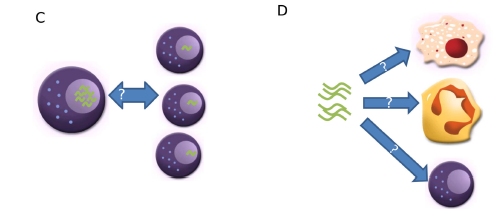
\includegraphics[width=0.7\textwidth]{figures/deconvolution_roles.PNG}
\caption{Sources of heterogeneity in biological samples.}
\label{fig:variability}
\end{figure}

In that context, numerical cellular deconvolution methods, by inferring automatically the composition of complex and highly-heterogeneous biological systems, are promising tools in the quest of the identification of causal drivers and understanding intricate biological mechanisms. 
}


\chapter{Cellular deconvolution}
\label{chap:deconvolution-state-of-the-art}

\section{Deconvolution objectives and main challenges}
\label{sec:deconvolution-challenge}

Over the years, the analysis of the transcriptome has substantially
contributed to our understanding of the processes involved in human
development and disease, but the complex nature of samples and tissues
under investigation has been largely neglected. Indeed, the mean
expression level of a gene differs between different cell subsets, while
in classic bulk transcriptomic analysis, only transcriptomic expression
averaged to the tissue level are provided. Finally, technical artefact
may confound the biological signal.

Additionally, the cell subset proportions themselves show high
variability between individuals, or even within a given tissue, driven
by physiological and pathological processes that induce \emph{cell
motility} and \emph{cell differentiation} (e.g infiltration and
differentiation of the monocytes into macrophages in reaction to a
tissue infection) \autocite{shen-orr_gaujoux13}. Therefore, observed changes in gene expression might
be the result of underlying differences in cell type proportions between
samples, biological differences due to clinical condition or a
combination of both \autocite{kuhn_etal12}.

One of the most common statistical analysis to identify key drivers of a
change in the biological condition is DGEA (differential gene expression
analysis), where in the most common case, we test whether the difference
of the mean expression of a given gene between two biological conditions
(often control versus disease) is statistically significant, with the
\emph{limma} R package being one of the most used
\autocite{smyth_etal22}. Analyses not accounting cell type composition as a confounding factor in
DGEA present suffer from three main drawbacks:

\begin{itemize}

\item
  If a cell population's proportion is correlated with the phenotype of
  interest, cell-subset agnostic DGEAs lose in \emph{specificity}, as
  they are prone to identify false positive differentially expressed
  genes. Ideally, differences due to biological condition should be
  decoupled from those resulting from a change of composition of the
  heterogeneous mixture.
  
\item On the other hand, differences in genes expression expressed by minor cell subsets may be masked by the high variation of the cell population
composition between samples or by the expression of the same gene in a
dominant cell type. This induces a dilution of the signal and a loss of
specificity. Indeed, in \autocite{whitney_etal03}, most of the inter-variability of gene expression within healthy patients was brought by a variation in the neutrophils
population, a largely dominant cell population in most biological
samples composing up to 70 \% of the total cell composition. 

\item As a consequence, not accounting for the cell composition makes it harder to determine the main causal driver of the biological dysfunction observed, especially the cell subset responsible for the observed signal, as illustrated schematically in \Cref{fig:deconvolution-confusing-variable}.
\end{itemize}

\begin{figure}
\centering
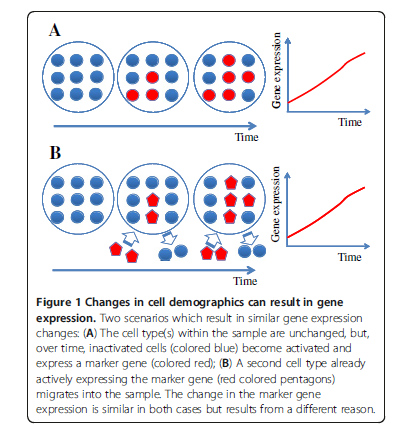
\includegraphics[width=0.7\columnwidth]{figures/dgea_cytometry_consequence.PNG}
\caption{Illustration, from an \autocite{shoemaker_etal12} example, of how two completely distinct causal drivers, result finally into the same global transcriptomic profile.}
\label{fig:deconvolution-confusing-variable}
\end{figure}


 





As suggested by \autocite{baker16}, along
with platform specific frameworks, incorrect data processing or other
technical batch effects, native heterogeneity of transcriptomics data
may explain the lack of reproducibility met currently . Indeed, several
studies have shown that the sensitivity and specificity of DGEAs
increases by integrating the cell population factor obtained from the
deconvolution of bulk expression Shen-Orr et al.
\autocite{shen-orr_etal10}. This is especially true
for highly heterogeneous tissues, such as peripheral blood composed of
many different immune cell subsets or tumoral tissues, with presence of
both normal and malignant cell types of possibly several stems.

Accordingly, the analysis of the interaction between the cell
proportions and the corresponding transcriptomic activity can help in
providing new insights in complex diseases, such as improving the
prognostic of a complex disease (probability of evolution to a more
severe form or to remission\ldots). For instance, an increase in the
proportions of oxyphil cells in the parathyroid gland is correlated to
the severity of the chronic kidney disease
\autocite{ding_etal20}. A reduced
proportion of neuronal cells in Alzheimer's patients increases the risk
of dementia \autocite{andrade-moraes_etal13}. On the other hand, computational methodologies, by decoupling
the sources of variability in heterogeneous data, can help in preventing
wrong associations between specific molecular marker (genes in
transcriptome-wide association studies (TWAS) or methylation CpG sites
in Epigenome-wide association study (EWAS)) to a phenotype of interest.
For example, some genes were down regulated in severe states of the
Alzheimer's disease in relation with a decrease in the number of neurons
expressing them and and not because of a causal biological mechanism
\autocite{mathys_etal19}.

%\begin{figure}
%\centering
%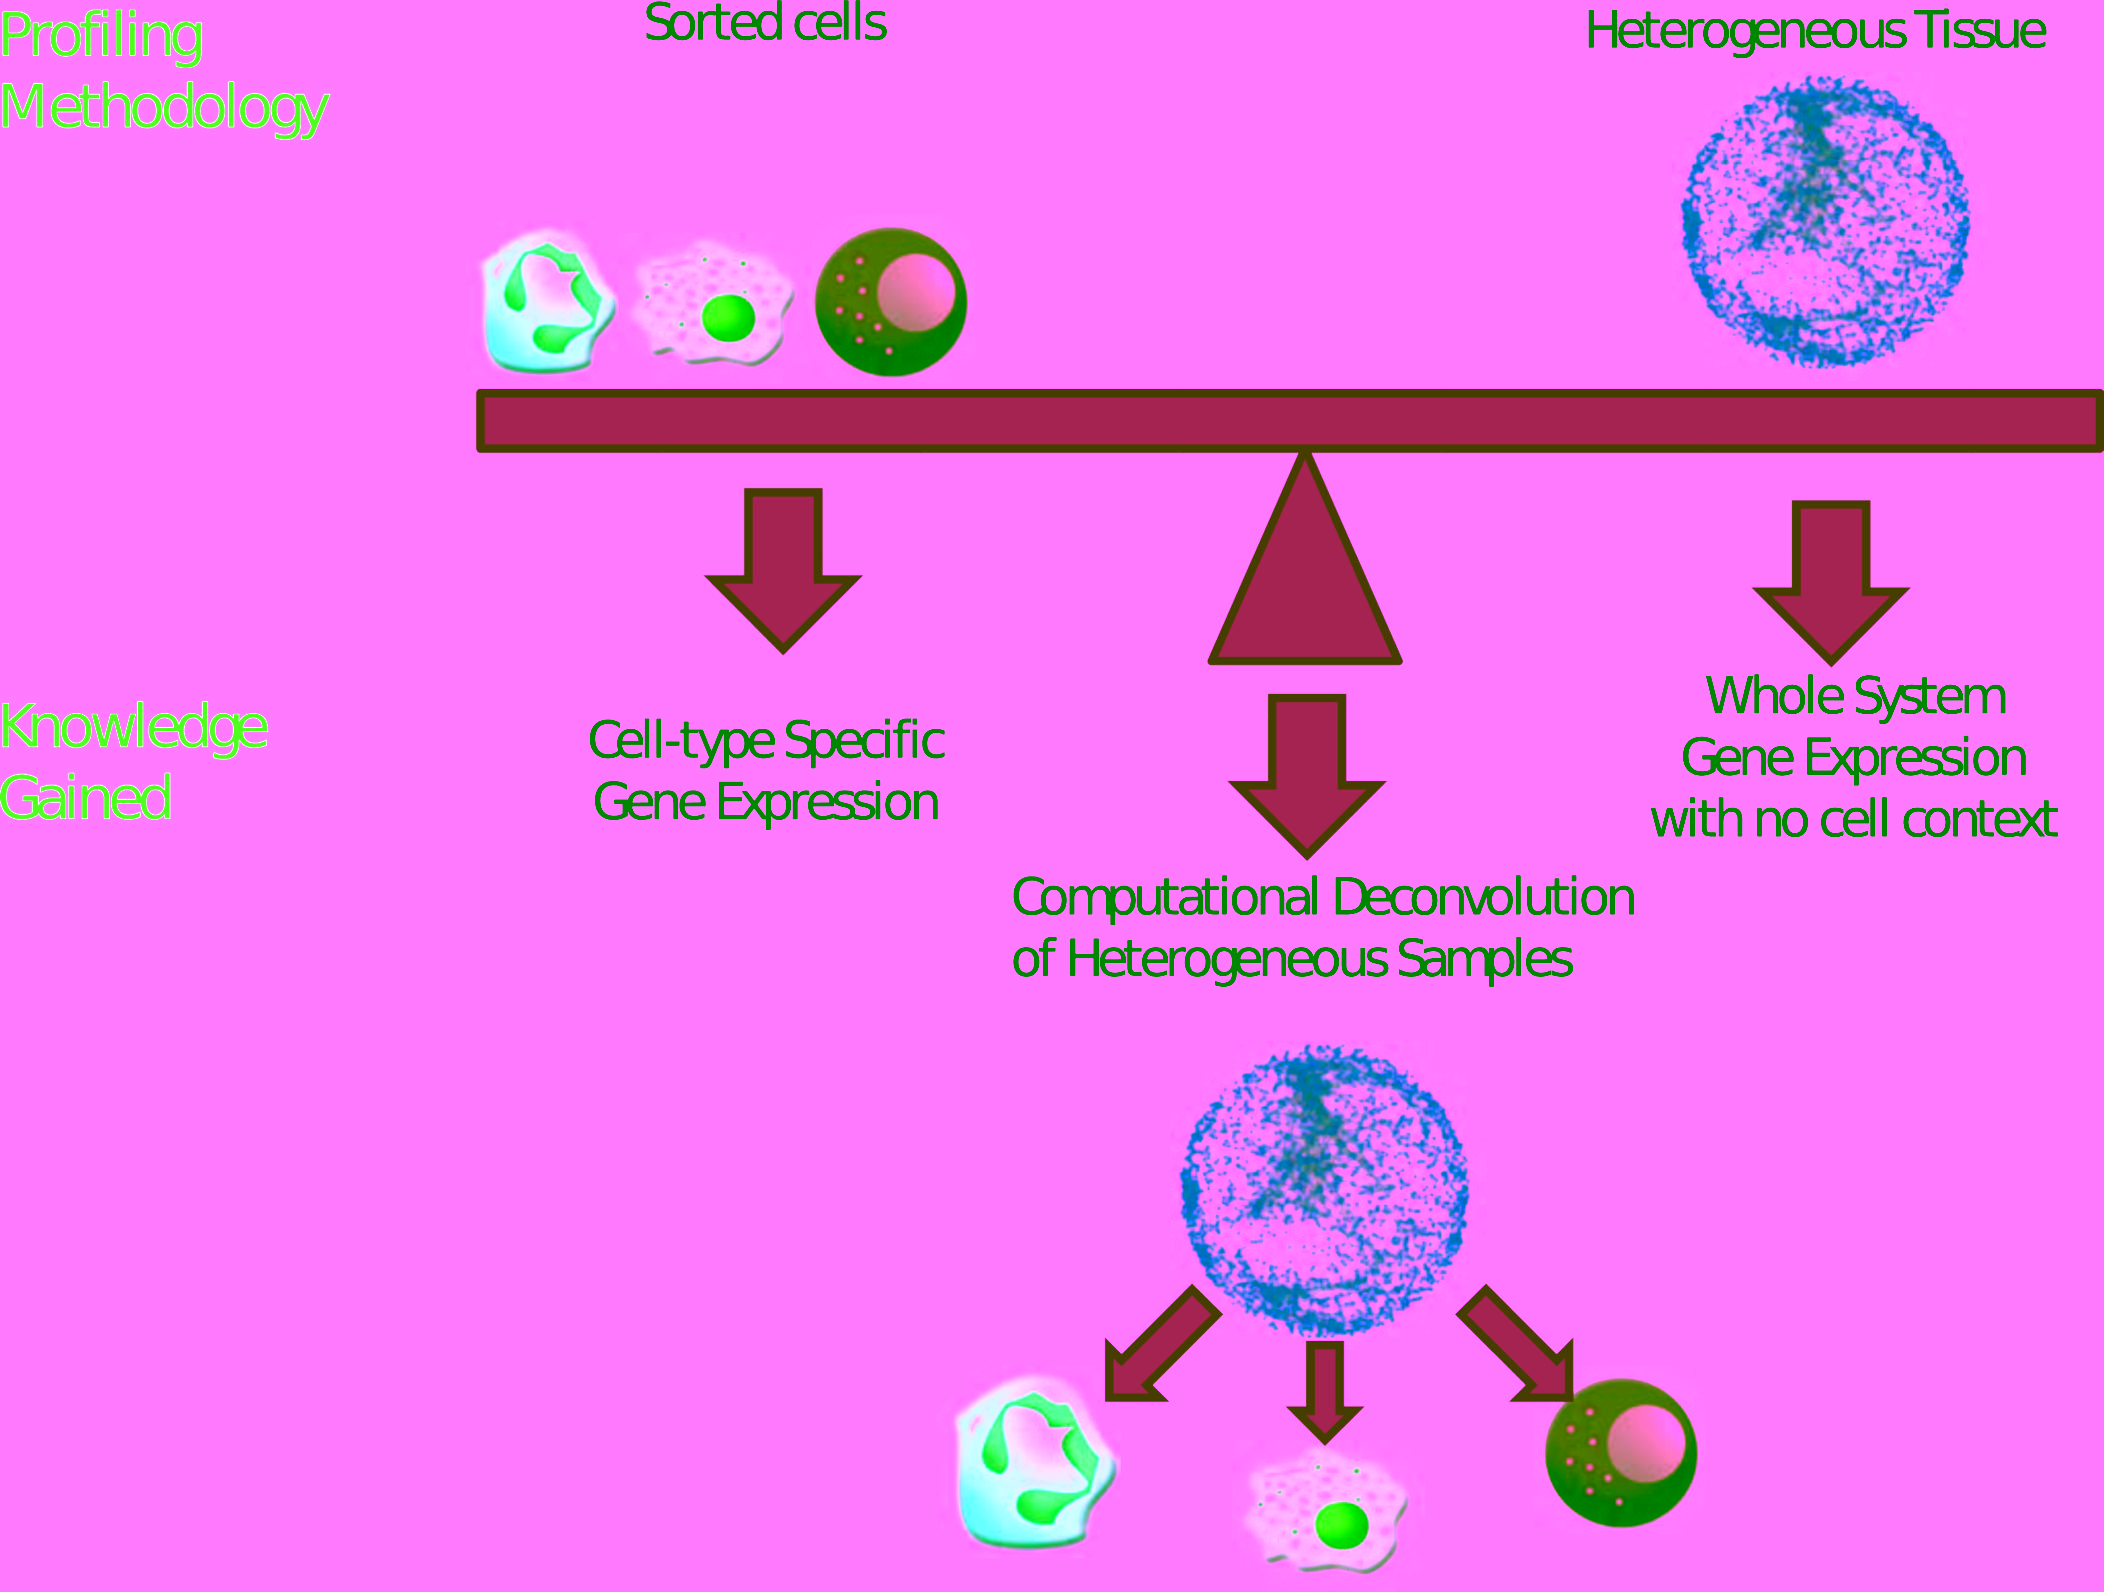
\includegraphics{figures/ShenOrr_2013_role_Computational_deconvolution.jpg}
%\caption{Computational deconvolution can capture both cell-centered and
%integrated biological network information}
%\end{figure}

\section{Physical methods}
\label{physical-method}


\subsection{Imaging methods}
\label{imaging-methods}

\emph{Immunohistochemistry}(IHC) \autocite{ju_etal13}, immune fluorescence (IF)
and in-situ hybridization (FISH-Flow, \autocite{kuhn_etal11}), as
opposed to the previous FACS method, enable an in-situ and so a spatial
characterization of the cell composition. They require tissue slides of
about one-cell width, such as FFPE samples, so that individual cells can
be visualized by microscopy at single-cell resolution. Individual cells
are first detected by segmenting the raw images, and then classified by
detecting signal emitted from the markers (can be present in nucleus,
cytoplasm or on within the membrane). To spot markers, both use a
combination of two antibodies: the primary one targets the cell marker
of interest while the secondary antibody, conjugated to either a
catalytic agent (IHC) or a fluorophore (IF), amplifies the signal. The
staining is then observed through a microscope and spatial
identification of the marked cell types is performed by pathologists or
with comparable performance by a deep deconvolution neural network. The
combination of different markers conjugated with a given antibody can be
used to unequivocally assign any stained cell to a specific population
\autocite{taube_etal18}.

Until recently, this methodology was limited to a small number of
markers due to the \emph{cross-reactivity} between primary and secondary
antibodies. The traditional way consists in staining consecutive tissue
slides with different antibodies. However, correctly realigning and
combining single slices is error-prone, losing the cell-cell distance
information. To overcome it, a recent methodology, the tyramide signal
amplification (TSA) system, allowed to increase the number of markers to
seven colours that could be stained simultaneously. In this system, TSA
free radicals catalysed by conjugation of the horseradish peroxidase to
the secondary antibody allows isolation of the complex formed by the
primary and secondary antibodies. It decreases then the risk of antibody
cross-reactivity when adding new antibodies to stain distinct markers.
In contrast to other methods, the multiplexed analysis of several
markers reveals in detail the anatomical structure, including cell
types' location, detection of lymphoid structures or formation of blood
vessels related to angiogenesis Lim et al.
\autocite{lim_etal18}.

%\begin{figure}
%\centering
%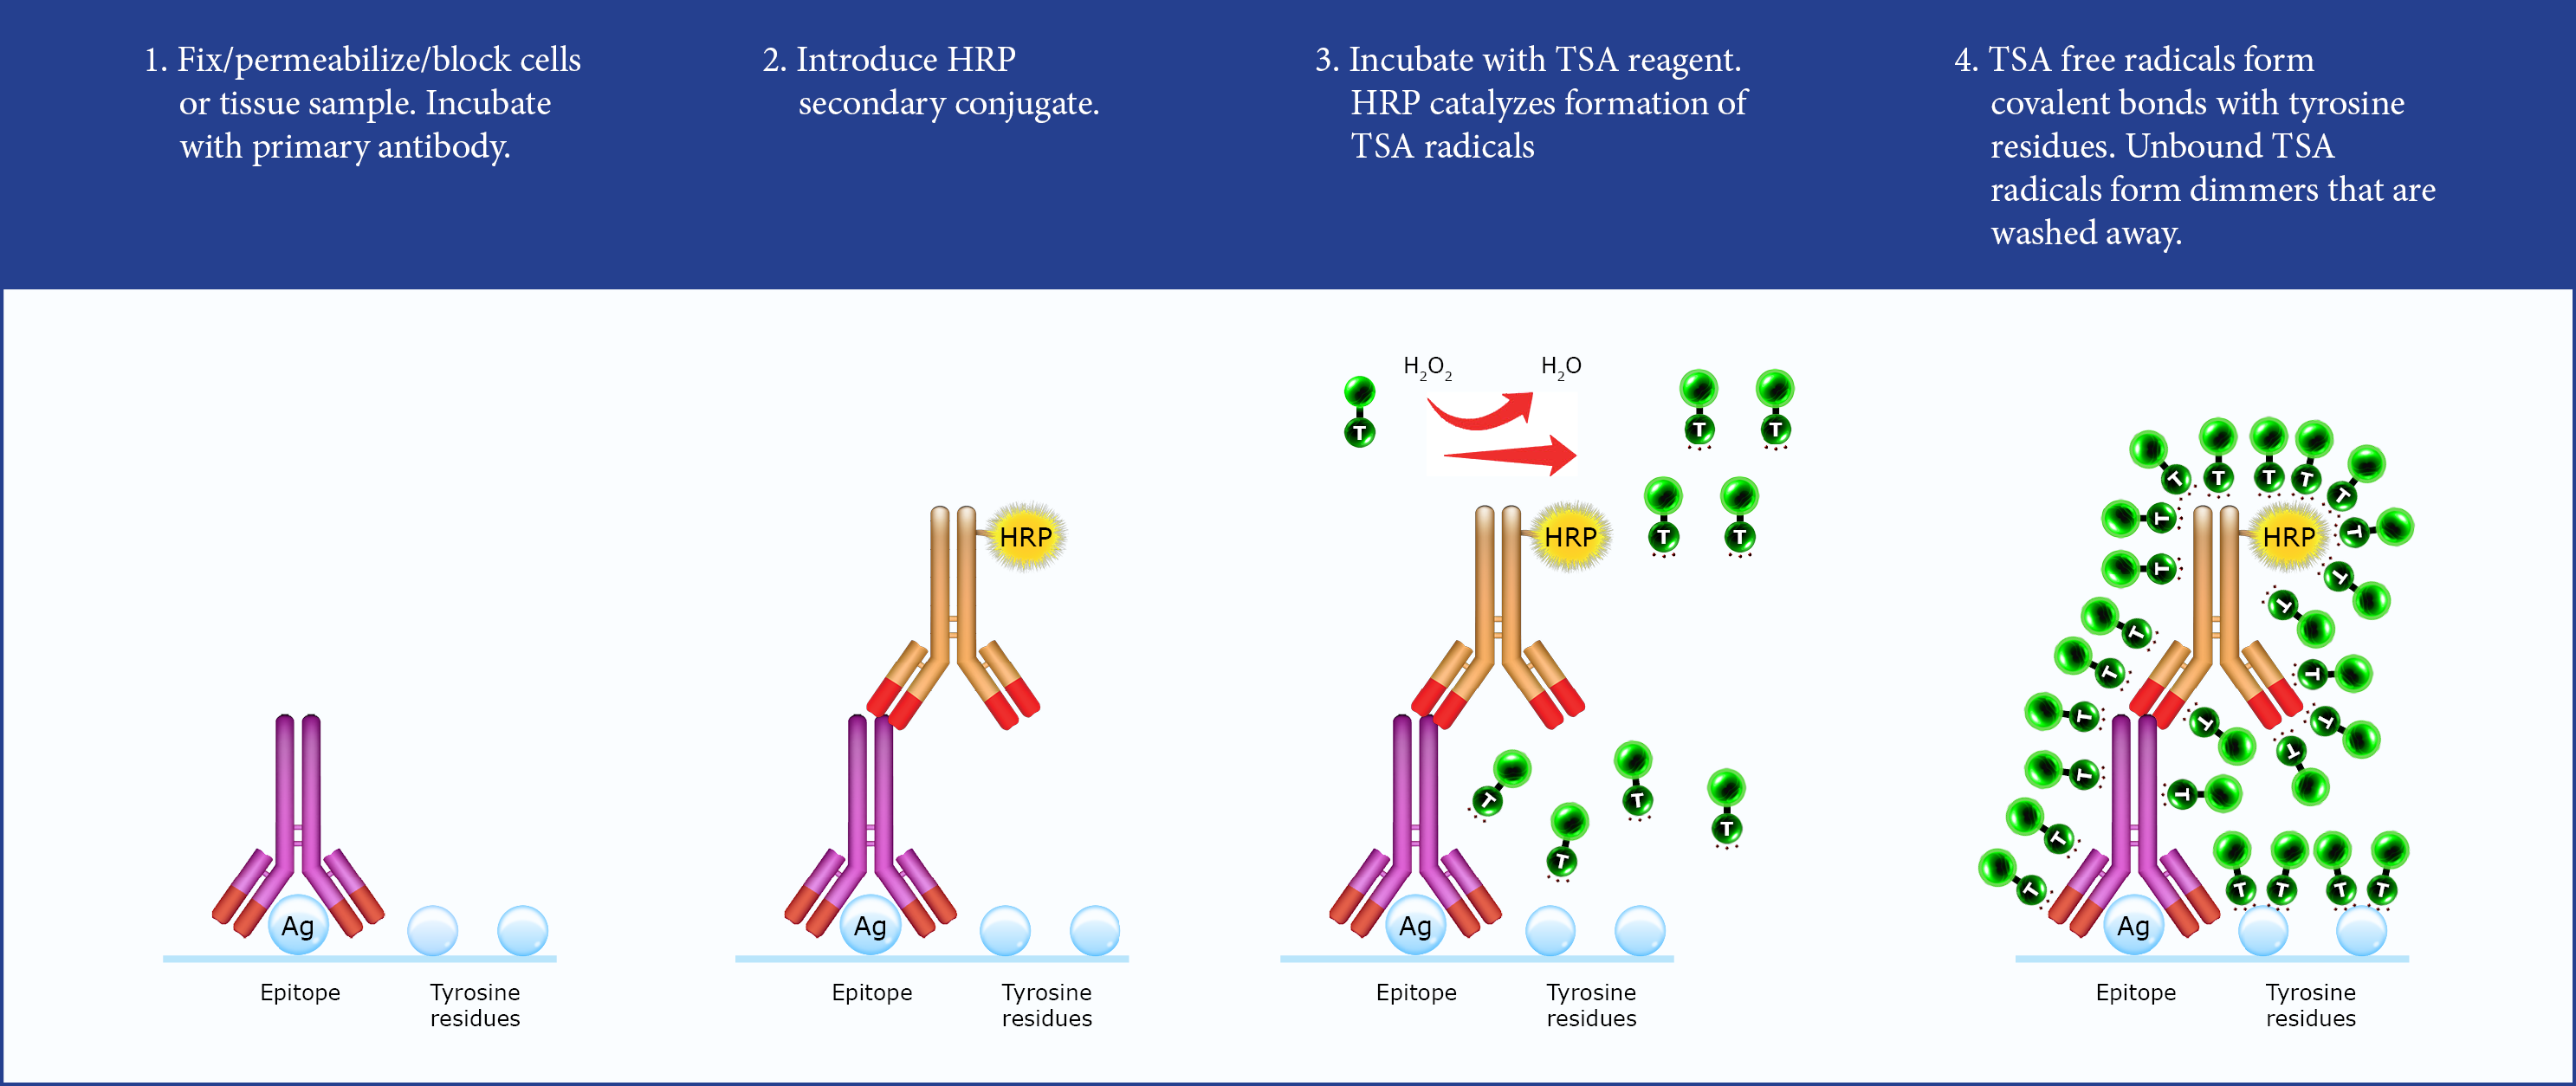
\includegraphics{figures/TSAWorkFlow.png}
%\caption{Description of TSA methodology}
%\end{figure}

Other IF-based methods that use a combination of sequential staining
with innovating staining approaches to enable highly multiplexed
quantification of biomarkers include cyclic immunofluorescence (CycIF)
\autocite{lin_etal15}, multiplexed immunofluorescence
(MxIF)\autocite{gerdes_etal13} and
multiepitope ligand cartography (MELC)
\autocite{schubert_etal06}. They
use photobleaching to stop cell fluorescence from the previous marker
and can stain 100 markers in a row. Finally, combination of mass
cytometry with IHC enable to get a deeper resolution at the subcellular
level (imaging mass cytometry (IMC)
\autocite{giesen_etal14}, Multiplexed
ion beam imaging: MIBI 33). Nonetheless, both technologies require heavy
instrumentation, with a weak throughput. Finally, a simpler technique named CODEX was
recently developed \autocite{goltsev_etal18} that requires less material to perform the analysis.

In-situ methods provide relevant yet highly dimensional data, with
information at single-cell level, including spatial coordinates and
staining intensities of the expressed markers up to the cell's
cytoskeleton. Spatial coordinates of the cell types can thus help to
detail the tumour immune landscape, for example, the cell-cell distances
yield information about the tumour immune architecture (vicinity of the
immune cell types) and so the tumour--immune cell interactions along
with their chronological evolution. To analyse this data, a similarity
matrix is built, representing the distances between two cell expression
profiles. Then, to interpret it, several dimensionality reduction
methods, such as t-SNE \autocite{maaten_hinton08} (non-parametric, unveil local structures) and UMAP (preservation of global distances)
\autocite{becht_etal19}, have been developed to reveal the
intrinsic non-linear structure of the single-cell data. Yet,
optimization of their hyper parameters, keeping both local and global
layout, is a complex task, and clustering of such 2D-projected plots may
be improved by accounting explicitly for the data sparsity
\autocite{pierson_yau15}. To
interpret the projections, instead of grouping cells with similar
expression profiles as homogeneous clusters, we may consider the recent
biological hypothesis that state of a cell is a continuum and that it
evolves dynamically throughout states, playing a key role on the
plasticity and so the ability of the immune system to respond quickly
and specifically to new pathogens or neoantigens. Graph-based approaches
can be used to infer linear and branched pseudo-temporal trajectories
that groups together cells emerging from the same lineage. Then, a
minimum spanning tree, or any other graph construction, some borrowed
from topological algebra, can be used to build a chronological timeline
of the cell state transitions, e.g.~the transition from naive to
cytotoxic CD8+ T cells. This estimated 1D ordering of time reference is
referred to as pseudotime. However, automatic extraction of information
from whole-slide images is still hampered by the numerous pre-processing
steps requiring manual interaction (such as defining the threshold to
discriminate unequivocally a marked cell type from background noise),
in-depth knowledge of image processing and extensive training of the
machine-learning algorithms. For instance, longitudinal single-cell
analysis helps disentangling the origin and the pseudo-time sequence of
distinct monocyte/macrophage states, with Monocle2
\autocite{qiu_etal17} revealing that
neither CX3CR1+ macrophages nor iNOS+ macrophages are present in the
early tumoral state.

\subsection{Cytometry analyses}
\label{cytometry-analyses}

Flow cytometry enables identification of populations at the single
level. To do so, the individual cells are isolated and then marked with
fluorophore-conjugated antibodies targeting markers of interest.
Identification of each cell's marker is performed by detecting the
fluorescence emitted back due to the simulation of a laser at a specific
wavelength. \emph{Gating}, namely the multiparametric expression of
various markers, can quantify precisely a large amount of single-cell
data (usually millions) within a large set of various population sets in
a relatively short time frame. The most recent FACS methods can quantify
up to 30 markers and 10,000 cells per second. FACS technics pioneered
the quantification of tumour-infiltrating immune cells, with early
description of dendritic cells (DC)
(\autocite{thurnher_etal96}) or
myeloid-derived suppressor cells (MDSC) (Veglia, Perego, and Gabrilovich
\autocite{veglia_etal18}).

\begin{figure}
\centering
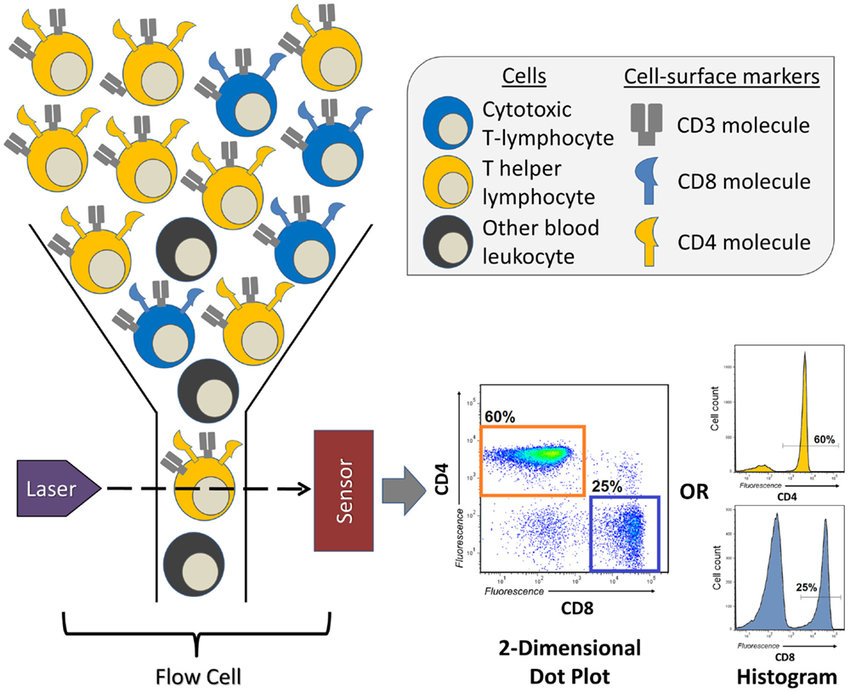
\includegraphics{figures/A-brief-overview-of-a-flow-cytometry-experiment-identifying-the-proportions-of-T-helper.png}
\caption{flow cytometry process}
\end{figure}

Initially, physical methods used to identify individual cells and hence
deduce their overall ratio in the biological sample were
Fluorescence-Activated Cell Sorting (FACS) or Laser Capture
Microdissection (LCM) technologies. However, these technologies require
specific cell-surface markers and corresponding antibodies to highlight
them. To overcome these limitations, novel systems relying on the
automatic discrimination of cell sizes by means of microfluidics or
dielectrophoretic separation were developed.

Of note, antibody-based methods require a known set of phenotypic
markers to uniquely identify cell populations, which might not be
available to set apart closely related cell population. As well, they do
not provide information about the functional state of specific immune
cells (no current consensus on single markers for determination of the
functional state e.g.~exhausted T cells)) and are biologically
intrusive, damaging cell structure (dead cells or doublets are not taken
into account). More specifically, FACS requires a large amount of
biological material while IHC provides only an estimate from a single
tissue slice.

To get a spatial insight on the transcriptomic activity, several
encouraging methods are developed to measure the expression of thousands
of genes in an antibody-free manner. This enables, using transcripts
instead of proteins, to characterize cells that can be identified only
accordingly to their transcriptomic activity. Two main classes of
methods use either hybridization (seqFISH+
\autocite{eng_etal19} and MERFISH
\autocite{chen_etal15}) or
sequencing (Spatial Transcriptomics
\autocite{stahl_etal16} and Slide-seq
\autocite{rodriques_etal19}). But
a compromise has to be found between the efficiency and the level of
accuracy required. SeqFISH and MERFISH enable subcellular resolution but
are low-throughput methods, while Spatial Transcriptomics can't achieve
single-cell resolution (\textgreater10 \(\mu m\)) while FISSEQ has a
high detection threshold (\textgreater200 mRNA molecules per cell).


\subsection{Single-cell technologies}
\label{single-cell-technologies}

The new Single-cell RNA sequencing ( \acrshort{scrna}) technologies are
promising to study rare populations, whose signal is usually confused in
bulk transcriptomics, and to get an insight on the intra-variability and
plasticity of the transcriptomic expression within a given population
\autocite{giladi_amit18}. First
step consists of isolating single cells, which can be done with plate-
(Smart-seq2, \autocite{picelli_etal13} via FACS technics or microfluidics-based (10X Chromium,
\autocite{zheng_etal17}) methods.
Microfluidics-based are less expensive, with higher throughput and can
thus profile a larger number of cells, but at the expense of lower
sensitivity. Then, each cell transcriptomic activity is individually
asserted. Besides, at the immune level, paired associations of the
\(\alpha\)- and \(\beta\)- chains forming the TCR determine together
their antigen specificity and are only kept at the single-cell level
resolution, along with the interaction between the immune population and
its functional state.

CyTOF \autocite{nomizu_etal94} is an
alternative method for the analysis of single cells is, in which
antibodies binding to the cell-surface-expressed proteins enable
unequivocal identification of the cell type. Cell content is then
ionised in a plasma state and analysed using a quadrupole time-off-light
(TOF) mass spectrometer. A higher number of simultaneously stained
markers compared to classical FACS can be used for the cell
identification.

However, their development is hindered by their expensive costs, complex
protocols and lack of statistical tools to interpret their results.
Additionally, the identification and composition determination of the
cell population may be biased
(\autocite{lambrechts_etal18}) as
some cell types are more likely to be damaged, and thus their total
expression underestimated. Doublets can also bias the expression, as
paired cells captured together generate hybrid transcriptome that might
be falsely interpreted as intermediate cell phenotypes. Indeed, the
primary step of single cell technologies requires a physical separation
and discrimination of the various cell subsets present in the sample,
subjected to the same artefacts and limitations of FACS methodologies.
Another main current limitation is the \emph{detection threshold} of the
transcriptomic signal, hindering detection of small transcriptomic
expression levels. This yields sparse transcriptomic expression
matrices, with numerous null expression values induced by
\emph{dropouts} due to the inefficiency of mRNA capture and the
stochasticity of mRNA expression. An additional challenge linked to the
peculiarities of these data is its intrinsic high dimensionality, with
higher noise and absence of biological replicates per sample. Finally,
annotation of the cell types is crucial but currently no consensus on
how to systematically identify known and novel cell types has been
established. Indeed, classical unsupervised clustering approaches split
the data into discrete clusters while cells are present in a continuum
of states, are sensible to the parametrization and might not identify
small clusters composed of rare cell populations. Accordingly, in most
of the  \acrshort{scrna} studies published so far, cell annotation is still
performed manually. A comparison between bulk and \acrshort{scrna} is illustrated below, in \Cref{fig:scrna-vs-bulk}.

\begin{figure}
\centering
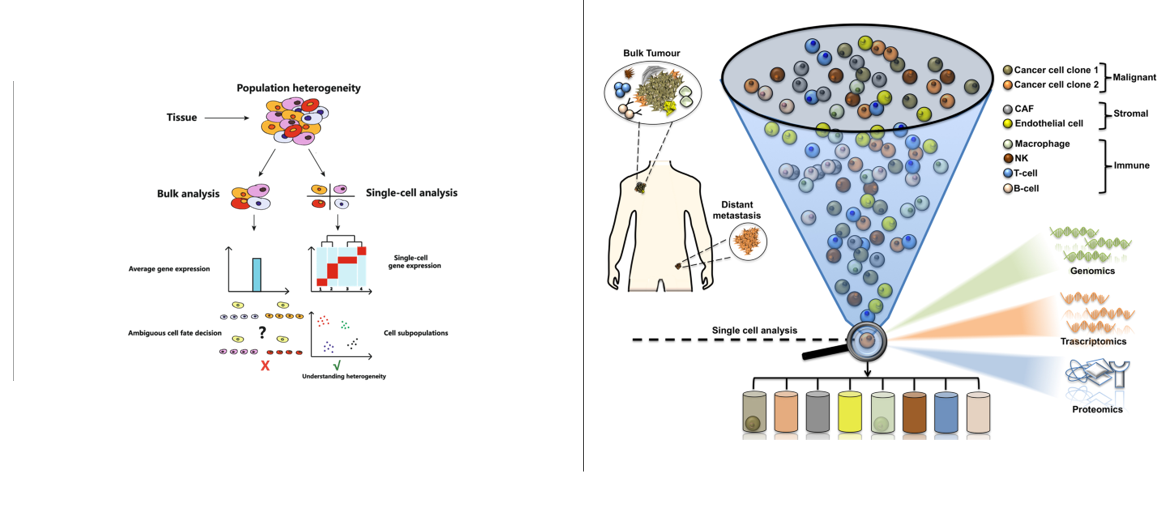
\includegraphics[width=0.8\textwidth]{figures/single_cell_methodology.PNG}
\caption{ Single-cell RNASeq pipeline compared to bulk transcriptomic RNASeq}
\label{fig:scrna-vs-bulk}
\end{figure}



A systematic and comparative review of the respective performance of these methods is summed up in \Cref{fig:mse-complex_heatmap}

\begin{figure}
    \centering
    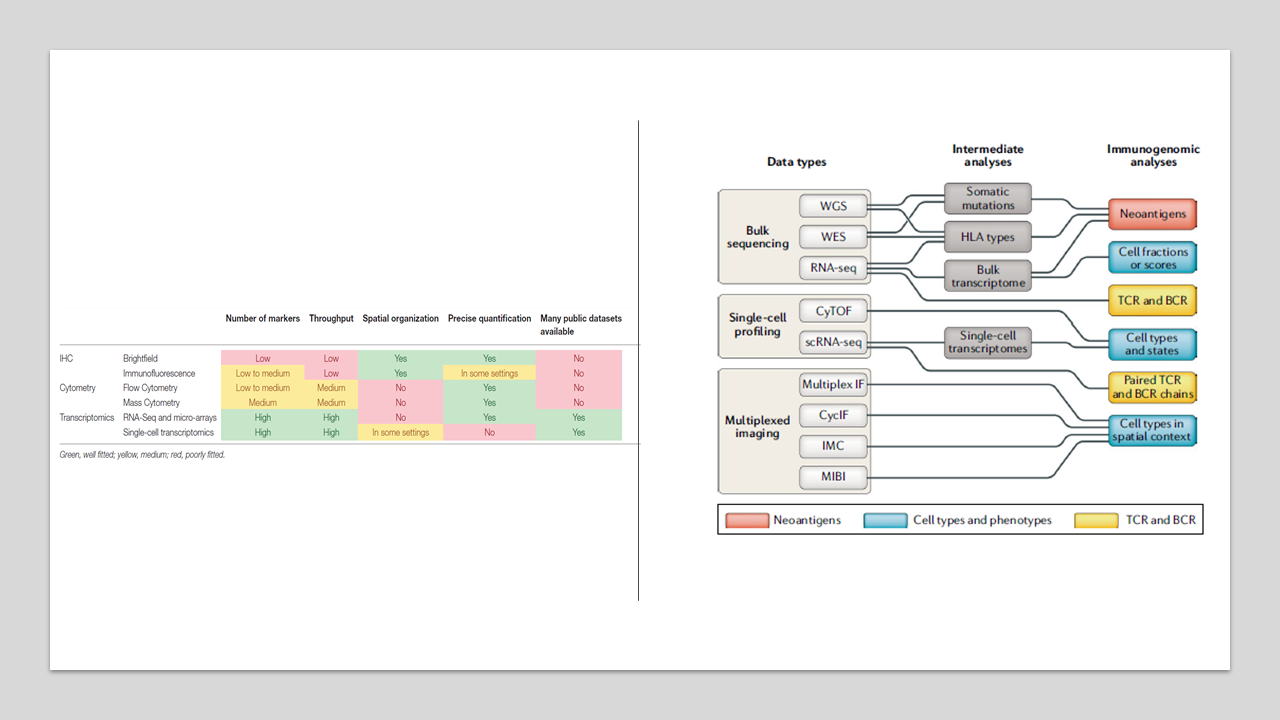
\includegraphics[width=0.5\textwidth]{figures/tme_estimation_technics.PNG}
    \caption{Comparison of accuracy and sequencing throughput of the most commonly used methods to decipher the biological medium, reproduced from \autocite{finotello_trajanoski18}}
    \label{fig:mse-complex_heatmap}
\end{figure}



\section{Computational methods using transcriptomics data}
\label{computational-methods-using-transcriptomics-data}

To overcome the highly costs of  \acrshort{scrna} technologies and exploit old
relevant bulk data (re diseases, long follow-up studies or complex
tissue extraction) for which the biological samples may not be available
anymore, multiple computational approaches have been developed in the
past years to infer ratios of cell types in biological
samples\autocite{avilacobos_etal18}. Additionally, single cell technologies, by physically separating
the various cell populations present in a biological sample, may hinder
the complex interactions within them, while computational techniques,
extracting directly cell-specific information from heterogeneous
samples, capture both cell-centered and whole-system information
landscape.

\emph{Deconvolution} generally speaking names the process that consists
in retrieving from a mixture its individual subcomponents. Linear
deconvolution is a subproblem of the general problem of the blind signal
separation, popularized as the `cocktail party problem'
\autocite{cherry53}. In a biological sample
(whole blood, tissue, \ldots), this consists generally in retrieving the
distinct cell populations (immune, stromal\ldots) composing it, but it
can be directly extended to identify the different sources of the RNA
production (for instance, many studies investigate on estimating a
tumour purity score returning the proportion of malignant cells in \autocite{yoshihara_etal13})
or set apart distinct cell phases. General pipeline is briefly described below \Cref{fig:cibersort-pipeline}

\begin{figure}
\centering
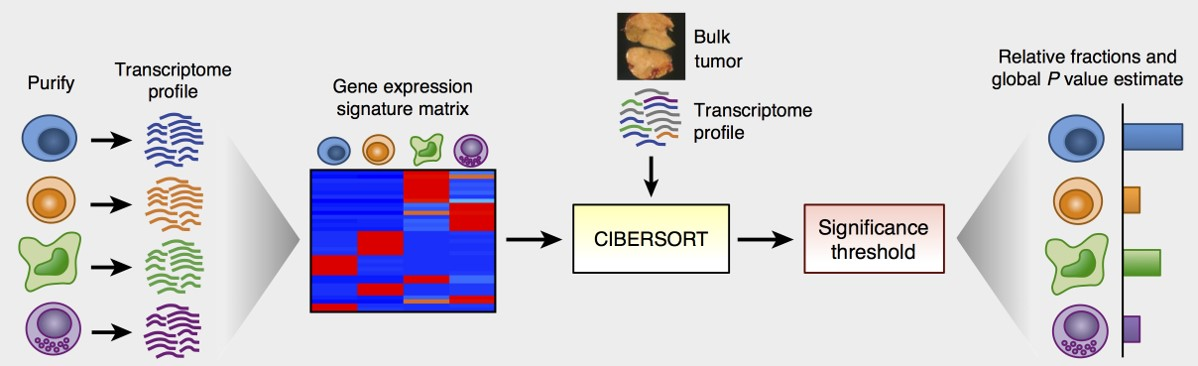
\includegraphics[width=0.7\textwidth]{figures/deconvolution_general_process.jpg}
\caption{Cibersort general description}
\label{fig:cibersort-pipeline}
\end{figure}

\todo{Use our own infography}

In classic linear deconvolution analyses, the gene expression measure is
the sum of each cell populations' gene expression weighted by their
corresponding proportions. If we consider a 'perfect' measure (no noise,
all cell types correctly identified, \ldots), we can be describe the
model as such:

\[
y_i = \sum_{j=1}^k x_{ij} \times p_j
\] 

with \(y_i, \quad 1 \le i \le n\) the sample's bulk transcriptome measure of gene \(i\), generated by \(k\) distinct cell populations
described by their proportion in the mixture \(p=p_{1:m}\) and their
individual specific expression \(x_{i, j}\), with \(1 \le j \le k\)
index of the cell population. Such equation states that the bulk gene
expression is the sum of individual cell specific expression \(x_{i.}\)
weighted by the proportion \(p_j\) of the cell population in the sample.
Additionally, the following constraints are generally applied on the model: 

\begin{equation}
\begin{cases}
\sum_{j=1}^J p_j=1\\
\forall j \in 1, \ldots, J, \quad p_j\ge 0
\end{cases}
\label{eq:simplex-constraint}
\end{equation}

 stating that no other cell population is present in the sample, and
that cell ratios must logically be non-negative values. For the ensemble
of \(n\) genes, this can be represented matricially by the following
equation: 
\[
y=\mathbf{X}p
\] 

Finally, let \(S\) the number of measured samples (in possible
distinct individuals, or in different tissues or at distinct period of
times in the same individual). The transcriptomic expression is then
given by a \(n \times S\) matrix, whose
\(s^{\text{th}}, \quad 1 \le s \le S\) is the transcriptome of sample
\(s\). Then the transcriptomic matrix \(\mathbf{Y}_{1:n, 1:S}\),
assuming that the expression of a population cell type is
\emph{tropic}-free (same no matter the individual or tissue) verifies
the following matricial equation: \[
\mathbf{Y}_{1:G, 1:N}=\boldsymbol{X}_{1:G, 1:J} \mathbf{p}_{1:J, 1:N}
\]

\[
\begin{pmatrix}
y_{1, 1} & \ldots & y_{1, N}\\
\vdots & \ddots & \vdots \\
y_{G,1} & \ldots & y_{n, N}
\end{pmatrix}
=
\begin{pmatrix}
x_{1, 1} & \ldots & x_{1, J}\\
\vdots & \ddots & \vdots \\
x_{G,1} & \ldots & x_{G, J}
\end{pmatrix}
\times
\begin{pmatrix}
p_{1, 1} & \ldots & p_{1, N}\\
\vdots & \ddots & \vdots \\
p_{J,1} & \ldots & p_{J, N}
\end{pmatrix}
\] where \(p_{j, s}\) is the proportion of the cell population \(j\) in
sample \(s\). Several information can be extracted from cell
type-specific analysis, to detect signal of a cell type in a mixture,
going further by estimating either its proportion or specific expression
profile or in a totally unsupervised manner, identify possibly new cell
populations by retrieving both individual signal and ratio of the
mixture. These four general information are summed up in the following
picture, and we describe in further details in next section main
technics used to do so.

%\begin{figure}
%\centering
%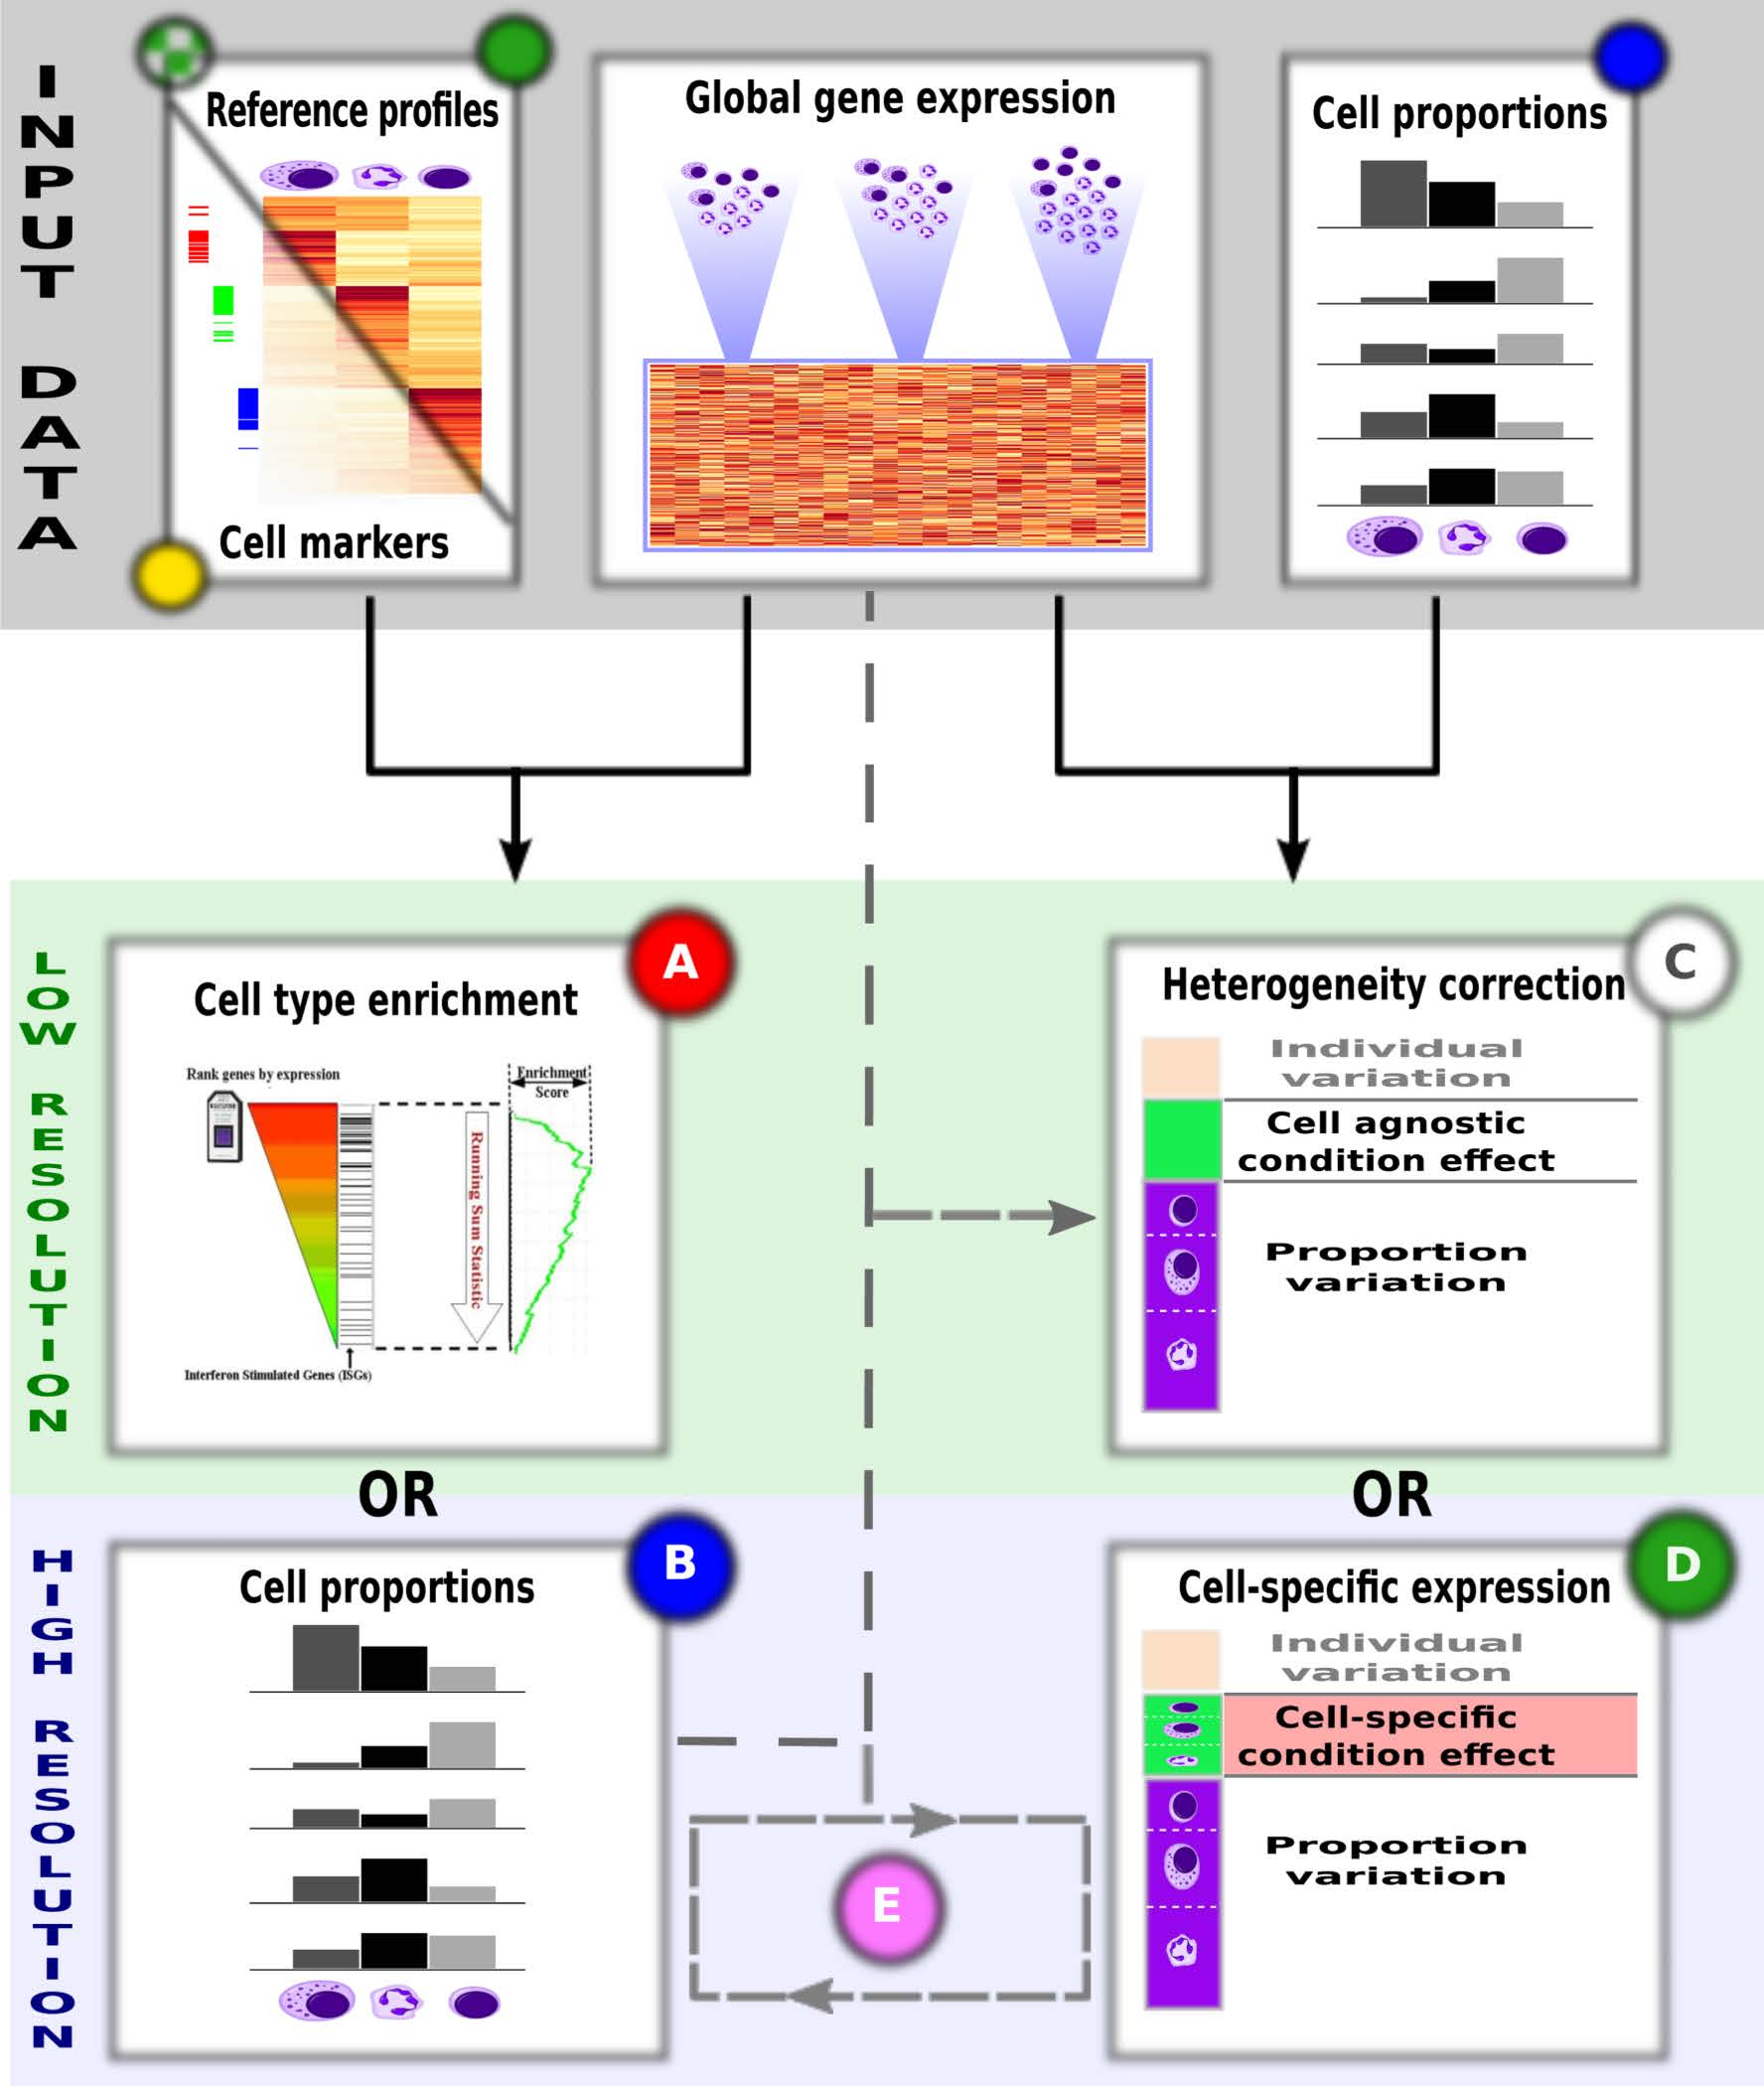
\includegraphics{figures/shenorr_purposes_deconvolution.jpg}
%\caption{Main purposes of computational deconvolution}
%\end{figure}


\subsection{Partial deconvolution technics}
\label{partial-deconvolution-technics}

Most published methods, referred as partial deconvolution methods, rely
on the measurement of cell proportions to estimate population specific
expression profilesStuart et al.
\autocite{stuart_etal04}, or on the measurement of
specific expression profiles to estimate proportions.


\subsubsection{Estimate the ratios}
\label{estimate-the-ratios}

In a perfect system without noise as modelled in equation {[}{]}, the
number of solutions, with \(p\) the unknown variable vector to estimate,
is given by the ``Rouché--Capelli'' theorem
\autocite{shafarevich_remizov13}. Briefly, uniqueness of the solution implies that the number of
genes \(n\) is equal to the number of cell types studies \(k\), and that
the expression of an individual gene can not be rewritten as a linear
combination of the remaining genes expressed in the sample (matricially,
this implies that the reference matrix \(\boldsymbol{X}\) is invertible).
When the number of genes exceeds those of cell populations, the system
gets overdetermined, and solution to the corresponding system of
equations, without collinearity in the gene observations, requires to
account for noise in the deconvolution problem.

According, goal of the ordinary least squares method (OLS) is to
minimize the sum of squares (SSE) between fitted values:
\(\hat{y} = \boldsymbol{X}\hat{p}\) and observed values: \(y\), regardless
of the distribution of the error term: \[
\hat{\mathbf{\epsilon}} = ||\hat{y} - y||^2 = ||\boldsymbol{X}\hat{p} - y||^2 = \sum_{g=1}^G \left( y_g - \sum_{j=1}^J \hat{p_j} X_{ij}\right)
\] The OLS estimator,\(\hat{p}_{\text{OLS}}\), that minimizes the sum of
residuals above, is given, using the normal equations, by: \[
\hat{p}_{\text{OLS}} = \arg \min_{\hat{p}} \left( ||\boldsymbol{X}\hat{p} - y||^2 \right) = (\boldsymbol{X}^T\boldsymbol{X})^{-1}\boldsymbol{X}^Ty, \quad y \in \mathbb{R}^n, \boldsymbol{X} \in \mathbb{R}^{n \times k}, p \in \mathbb{R}^k
\] \[
\hat{\mathbf{p}}_\text{MLE} = \arg \max_{\mathbf{p}} \left( \mathbb{P}_\mathbf{p} (y_{1:G}|\boldsymbol{X}_{1:G, 1:J})\right)= \arg \max_{\mathbf{p}} \left( \prod_{g=1}^G  \mathbb{P}_\mathbf{p} (y_{g}|\boldsymbol{X}_{.g})\right) \text { with } y_{1:G} \sim \mathcal{N}_G(\boldsymbol{X} \mathbf{p}, \sigma^2\mathbf{I}_G)
\] We generally assume a null spherical multivariate Gaussian
distribution for the distribution of the noise, a.k.a. the \emph{error
term}
\(\mathbf{\epsilon} \sim \mathcal{N}_n (\mathbf{0}, \mathbf{\Sigma})\),
with a \(n\)-zero mean vector and a diagonal covariance matrix of
constant diagonal term corresponding to the variance on the gene
measure, \(\mathbf{\Sigma} = \sigma^2 I_n\). The form of the covariance
matrix induces several assumptions on the biological model:

\begin{itemize}

\item
  \emph{weak exogeneity} the cell type-specific expression profiles are
  considered as fixed values and not random variables. This erases the
  intra-variability of a given gene within a cell population.
\item
  \emph{constant variance} as homoscedasticity, meaning that the
  variance is the same for any observation, in other terms, that
  \(\text{var} \left(\epsilon_i\right)=\sigma^2, \quad \forall i =1, \ldots, n\)
\item
  \emph{independence of the errors},
  \(\quad 1 \le i \le n, \quad 1 \le j \le n, \forall i \neq j, \quad \text{cov} (\epsilon_i, \epsilon_j)=0\),
  implying biologically that the bulk gene expression measured is
  independent of the others
\item
  the null expected value of the error term,
  \(1 \le i \le n, \quad \mathbb{E}(\epsilon_i)=0\), implying
  biologically that only the cell populations referenced in the
  signature matrix are responsible for the observed transcriptomic
  expression.
\end{itemize}

To avoid redundancy and guarantee the uniqueness of the solution, the
reference matrix \(\boldsymbol{X}\) must be of full rank \(k\), implying
that the number of gene observations \(n\) is superior to the number of
cell ratios to be estimated \(k\), and that no cell population specific
expression can be written as a linear combination of the others
(multicollinearity). The lowest variability on the estimate is obtained
when cell expression profiles are uncorrelated to each other, a strongly
assumption that might be only valid at a high level of the cell lineage.

With the conditions listed below, we can apply the
\emph{Gaussian-Markov} theorem, stating that the OLS estimate is not
only the unique estimate returning the global minimal of equation
{[}{]}, but the BLUE estimator (best linear unbiased estimator),
i.e.~the unbiased estimator (in average, no difference between the
estimated parameter and its true value) with the lowest variance. Except
when the number of ratios to estimate is rather small (and so the
columns of reference matrix profile), the direct computation of the
reverse matrix \((\boldsymbol{X}^T\boldsymbol{X})^{-1}\) is a rather difficult
task, proned to numerical rounding errors. Instead, \(QR\)
decomposition, in which the rather difficult reference matrix
\(\boldsymbol{X}\) is decomposed as the product of \(\mathbf{Q}\), a
\(n \times k\) orthogonal matrix, and \(\mathbf{R}\), a \(k \times k\),
upper triangular matrix, is often favoured. The OLS estimator is then
given by: \(\hat{p}_{\text{OLS}} = \mathbf{R}^{-1} \mathbf{Q}^T y\),
where the triangular matrix \(\mathbf{R}\) is much easier to invert.
Additionally, in the LLS method, linearity is only required with respect
to the coefficients of the model \(p\) with a possibly nonlinear
transformation of the bulk transcriptome \(y\) and gene reference
profile \(\boldsymbol{X}\): \[
\psi'(y_i)= p_0 + \sum_{j=1}^k p_j \psi_j(X_{ij})
\] with \(\psi\) a possibly nonlinear function. Usual transformation is
the TPM normalization for \acrshort{RNA-Seq} data that enforces a fixed measured
quantity of RNA transcripts for each sample. As shown in
\autocite{racle_etal17}, TPM
normalization being a linear function ensures that if the sum of the
estimated ratios in raw data sums to one, then the TPM normalized
estimated ratios comply this condition. Another rarer function used is
the \emph{log2} transformation
\autocite{hoffmann_etal06},
supposed to guarantee better the normality conditions of the residuals
required by the Gaussian Markov theorem. However, this model has no
biological sense, with no sum-to-one constraint preserved.

This \emph{linear model} is the one used in
\autocite{abbas_etal09}
paper, using the R \emph{lsfit} function, to estimate 18 different
immune cell ratios. They show that the activation of NK and T helper
lymphocytes were highly correlated to symptoms of the SLE disease, with
a prominent impact on the interferon signature. But it is sensitive to
outliers and efficiency of the estimate relies on a set of strict
conditions that aren't usually met in biological conditions,
e.g.~homoscedasticity of the residuals and absence of correlation
between the residuals and observed values. Additionally, the OLS
estimated ratios might be negative or not sum-to-one, having no
biological sense. Hence, such coefficients are artificially removed
after the estimation. The same method is used in
\autocite{li_etal16}, in a context of
tumoral mixture. To avoid accounting for tumoral cells when asserting
ratios of infiltrated cells, only genes both highly correlated to the
cell types of the sample and negatively correlated to the \emph{tumour
purity} are integrated in the reference matrix. In this study, tumour
purity is the ratio of \emph{aneuploid cells}, namely cells with a non
canonical number of 46 chromosomes, asserted by the CHAT (clonal
heterogeneity analysis tool) R package (not maintained anymore on the
CRAN), considered as surrogate variable of the true ratio of tumoral
cells. Additionally, a pre-filter on the top \(1%
\) most varying genes is performed to maintain the heteroscedascity
assumption. This study identifies 2 subgroups of melanomas with two
distinct levels of TCD8 subsets, and associated to distinct prognostic
issues.

The sum-to-one ratios might be relaxed, by integrating an additional
constant term accounting for remaining cell populations that might have
been left undetected. To do so, we simply need to add a column of ones
in the reference cell matrix is now:
\(\boldsymbol{X} \in \mathbb{R}^{n} \times \mathbb{R}^{k + 1}\), and
\(k + 1\) cell ratios are now estimated, \(p_0\) being the cell ratio of
uncovered cell subsets present in the mixture. Finally, a direct
approach, by adding weights proportional to the influence desired for
the gene expression measure on the OLS estimate, or indirect robust
approach adjusting automatically to outliers, can be used to account for
outliers in the mixture. In the weighted approach, the Weighted Least
Square estimate is given by
\(\hat{p}_{\text{WLS}} = (\boldsymbol{X}^T\mathbf{W}\boldsymbol{X})^{-1}\boldsymbol{X}^T\mathbf{W}y\)
with \(\mathbf{W}\) the diagonal matrix of weights, hence, the
individual error estimate with an intersection term is given by
\(\hat{\epsilon_i}=w_i\left( y_i - \hat{p_0} - \sum_{j=1}^k \hat{p_j} X_{ij}\right)^2\).
The weights are given by the user, low-quality points being associated
to small weights. In the robust approach, the weights are iteratively
adjusted till convergence (the usual prior being usually the uniform
weight for each observation), or, in a stricter way, some genes are
simply not used for the estimation.

CellPred, developed in \autocite{wang_etal10} for the estimation of stromal and tumour proportion from
microarray transcriptomic data, is an user-friendly web service that
performs a multivariate linear regression model with a noise intercept.
EPIC, \autocite{racle_etal17},
includes both processes, for the estimation of cell ratios in a tumoral
context. Instead of a constant term accounting for none described cell
population, the algorithm assumes that genes expressed in tumoral cells
are poorly transcribed in immune or stromal cells, and an additional
column corresponding to tumour is added to the reference cell
population. The signatures in EPIC were developed using both bulk and
 \acrshort{scrna}-seq data from circulating and tumour-infiltrating immune cells,
CAFs and epithelial cells, with one designed for whole-blood samples and
another for solid tumoral tissues. Besides, a weighted LLS method is
implemented to retrieve the ratios, with less weight given to highly
variable genes. It's worth noted that this method can be applied to
\emph{solid tumours} as the immune cells do not mix up with tumoral
cells, but not hematological malignancies (lymphonenia, leukemia\ldots),
where the estimated immune cell subset may be composed of a mixture of
both normal and mutated cells.

Same approach, but simply using a constant intersection term, is used in
the quanTIseq algorithm
\autocite{finotello_etal19}. To
integrate the drop-out observed in some cell subsets poorly present in
the sample and highly correlated to other cell types, they implement a
heuristic strategy averaging the estimated ratio of Tregs in presence
and in absence of the highly correlated \(TCD4^+\) subset in the design
matrix. QuanTIseq is specifically tailored for RNA-seq data and
implements a full analytical pipeline, from pre-processing of raw
RNA-seq data until deconvolution of cell fractions.

Actually, with gene expression data normalized per sample et cell
population, the estimated ratios \(\hat{p}\) returned by the
deconvolution method correspond actually to the fraction of mRNA coming
from each cell type, rather than the cell proportion itself. Dividing
the number of transcripts associated to a cell subset by the average
production of RNA transcripts (or equivalently the total weight of RNA)
yields the expected number of cells associated to this compartment.
Finally, the true cell population ratio derived from the RNA fraction is
given by: \[
\hat{p^*_j} = K \frac{\hat{p_j}}{r_j}, \quad K= \frac{1}{\sum_{j=1}^k \frac{\hat{p_j}}{r_j}}
\] with \(r_j\) the average number of transcripts extracted per cell
type, and \(K\) a normalization constant, such that the modified
estimated cell ratios still sum to one.

Post-correction of this biased effect is taken into account in
\autocite{racle_etal17} and \autocite{finotello_etal19}
studies, using the RNAeasy mini kit (Qiagen) to extract RNA nucleotides
a and a Fragment Analyser (Advanced Analytical) to quantify it in
\autocite{racle_etal17} paper and
using as a surrogate variable the expression of the housekeeping genes
in the Proteasome Subunit Beta 2 (PSMB2)
\autocite{eisenberg_levanon13} in \autocite{finotello_etal19} to retrieve 
the average number of transcripts \(r_j\). Still,
extraction efficiencies evaluated by both methods are high correlated.

Another similar interpretation of the \(r_j\) coefficient, as reported
in \autocite{liebner_etal14}, is the correction for technical bias with differential RNA
extraction efficiency whether the cell type. Unlike EPIC and QuantiSeq,
the MMAD (microarray microdissection with analysis of differences)
algorithm does not consider the coefficient extraction efficiency as
data provided by the user as input, but rather as a parameter to
estimate for the deconvolution algorithm, as well as the potential
biological perturbation induced by the phenotypical condition of the
sample. Then, the true estimated cell ratio can be decomposed, and
directly plugged in the LTS regression (ref equation): \[
\hat{p_{js}}^*= \hat{r_j} \hat{\beta_s} \hat{p_j}
\] In this case, the linearity between the response variable and the
weighted combination of the estimates is lost, and the LTS estimate is
computed using a non-linear conjugate gradient search algorithm,
implemented in MATLAB, with additional non-negative constraint on the
estimated parameters.

In the previously described approaches, all genes that were measured in
both the transcriptome \(y\) and the reference profile \(\boldsymbol{X}\)
were used for the deconvolution. However, such a an approach may yield
biased estimates, as the expression of some genes might significantly
differ between the bulk mixture and cell-separated subsets. Yet, these
outlying genes are the ones having the largest influence on the fit, due
to the squaring distance used to compute the error term.

Therefore, robust least-squares regression use only a subset of these
genes. To evaluate these methods, two metrics are generally used: the
relative \emph{efficiency} of the robust estimate, compared to the OLS
estimate when the assumptions of the Gaussian-Markov theorem apply (the
OLS estimate is indeed asymptotically efficient estimate, in the sense
of attaining the Cramér--Rao bound ), and the breakdown point (BP),
which is the minimal proportion of outliers in the dataset required so
that the estimate does not converge anymore. The OLS estimate has a
small BP of \(\frac{1}{n}\), implying that one single unusual
observation makes the estimation divergent
\autocite{rousseeuw85}. Several robust
methods, making a compromise between efficiency and robustness of the
estimate, were developed:

\begin{itemize}

\item
  M-estimate replaces the LLS criterion with a robust function of the
  residuals, giving less weight to highly leveraged points {[}{]},
\end{itemize}

\[
\hat{p}_{\text{IWLS}} =  \arg \min_{p} \sum_{i=1}^n \rho\left(\frac{y_i - \sum_{j=1}^k \hat{p_j} X_{ij}}{\hat{\sigma}}\right) = \arg \min_{p} \sum_{i=1}^n \rho\left(\frac{r_i}{\hat{\sigma}}\right)
\] 

where \(\psi = \rho'\) is the derivative of the robust function
\(\rho\), called the \emph{influence function}, for which the null
argument is the estimate to be found, and \({\hat{\sigma}}\) an estimate
of the residuals variability (sometimes the mean absolute deviation is
used), then \(\frac{r_{1:n}}{\hat{\sigma}}\) is the vector of
standardized residuals. With \(\rho(t)=\frac{1}{2}t^2\), we return on
the original OLS problem. Huber's function was the first used, in 1981,
with a strong smoothing as any absolute residual going beyond a constant
\(c\) (set to 1.345, the efficiency is \(95\%\) worth of the OLS
estimate) is given a null weight, while the same weight is given to any
other residual. Tukey's bisquare function is a soft smoothing function,
with the following influence function:
\(\psi(t)= \max \left(0, \left(1 - (\frac{t}{c})^2\right)^2\right)\).
Observations associated with a strong residual and so far the regression
line are given less weights, and the threshold gives null weight to
points that are farther from the regression line from what would be
expected by random chance. With c\(c=4.6885\) the efficiency of the
estimate is the same as Huber's estimate. With both functions, the
weights for each observation depend on the residuals that depend
themselves on the weighted estimator which itself is dependent of the
weights. As a result, the robust estimator must be computed iteratively.
The general process consists first in the initialisation step in
computing the OLS estimate, assuming uniform weights for any observation
(or any other weight returned by robust estimator, as in MM-estimates,
\autocite{yohai87}). Then, each observation
is weighted by the transformation of its corresponding residual value by
the influence function, and a weighted regression is performed, as given
in equation {[}{]}. When the weighted estimate converges, we stop this
iteratively reweighed least square regression. Although not described in
any deconvolution paper, the standard \emph{rlm} (for robust linear
modelling) function in the R MASS package, that performs the Tukey's
biweight iterative regression, is often implemented as a standard robust
method in any deconvolution benchmark paper. Another influence function
implemented is the Least absolute deviation (LAD), aka the \(L_1\)
estimate, that minimizes the absolute difference of the residuals,
instead of the squared differences:
\(\hat{p}_{\text{MAE}} = \arg \min_{\hat{p}} \left( |\boldsymbol{X}\hat{p} - y| \right)\).
Accordingly, extreme gene expression values \(y\) have less influence on
the regression. However, LAD can not be solved analytically, requiring
an iterative approach, such as the simplex-based Barrodale-Roberts
algorithm \autocite{barrodale_roberts73}. A LAD regression is performed in the RCR (robust
computational reconstitution) algorithm supplied in
\autocite{hoffmann_etal06}, in
which additionally trimming is performed (cf next point) and where the
non-negativity and the sum-to-one constraints are enforced. The final
number of genes used in their trimmed regression process corresponds to
the minimal number of genes to guarantee the uniqueness of the solution
(no matter the initial ratio estimates given in the initialisation
process, the same estimate is returned). Interestingly, they showed
theoretically that adding additional gene measures from the mixture at
that trimming point, that are more likely to be uncorrelated with gene,
leads to an artefact, with equal ratios attributed for each cell
population. All these methods remain sensitive to high leverage outliers
present in the cell reference matrix, and thus have the same breakdown
point as the OLS estimate. Additionally, they are less efficient in the
best case where the error is normally distributed, with LAD having the
lowest efficiency of 0.64 compared to the OLS estimate. - The LTS (least
trimmed squared) method was first proposed in
\autocite{rousseeuw85}, in which the
purpose is to find the \(q= n(1- \alpha) + 1\) observations, with
\(\alpha\) corresponding to the proportion of trimming, that have the
smallest residuals. Practically, the estimate is given by: \[
\hat{p}_{\text{LTS}} =  \arg \min_{p} \sum_{i=1}^q r_i (p)^2
\], with \(r_i (p)\) the residuals ordered by increasing order. LTS has
a strong BP of 0.5, taking \(\alpha=\frac{n}{2}\), making it strongly
resistant to outliers, but a very low efficiency of 0.08. LTS is an
NP-hard problem \autocite{rousseeuw85},
as any combination of \(\binom{n}{q}\) observations should be tested, to
find the \(q\) observations for which the estimate is minimal. With a
large number of observations, that's not computationally feasible, hence
\autocite{rousseeuw_vandriessen06} proposed a stochastic faster version of this algorithm,
in 2006. However, its performance is highly dependent on the initial
random \(q\)-subset chosen, and it's still too slow when the sample size
is too big, with initial bad initialization. Eventually, the number of
outliers to be trimmed has to be provided by the user. Accordingly, the
FARDEEP algorithm was developed by
\autocite{hao_etal19}, returning an
adaptive LTS estimate. At each step, the total number of points
considered as outliers is bounded between an overestimate and an
underestimate of the total number of outliers, with the series of
overestimate strictly decreasing and the sequence of underestimate
strictly increasing. Thus, the algorithm is guaranteed to converge in a
fixed number of steps, according to the hyperparameters provided by the
user. However, the algorithm is highly sensitive to the tuning parameter
\(k\) that indirectly controls the final number of observations trimmed
during the regression, and is not easily interpretable (the set of
outliers is composed of the observations for which the corresponding
absolute residual is above the median of the residuals multiplied by
\(k\)). And there's no theoretical result on the efficiency or even on
the consistency of the estimate returned, especially no guarantee to
find either the true number nor the set of outliers. A review of robust
linear estimates is supplied in \autocite{yu_etal14}, with 10 methods benchmarked, and in which
MM-estimates and REWLSE estimates have overall the best performance in
terms of robustness and asymptotic efficiency.

SVR (support vector regression) uses as well a specific metric keeping
the most informative gene expression, but rely on a different paradigm
than robust linear regression. As in classical linear regression, linear
SVR identifies the hyperplane that fits as many data points as possible.
But contrary to classical linear regression approaches, where all
observations are used for the fitting process, or to robust linear
approach, where distant points are trimmed or given less weight, the
most relevant gene expressions, referred as ``support vectors'' (SVs),
are the ones the most distant from the fitted hyperplane (in 3D, those
lying outside a tube of radius \(\epsilon\), centred on the fitted
hyperplane). SVs, penalized by a slack variable \(\zeta_i\) according to
their distance from the \(\epsilon\)-tube, define alone the linear
function, and any gene expression altered within the \(\epsilon\)-tube
would not impact the regression curve. Generally, the metric used in SVR
approach complies with the statistical learning principle stating that
in order to obtain a small risk, both the training error and model
complexity must be controlled. Hence, the optimization function consists
in \emph{a loss term} to be minimized (herein, the difference between
the estimated and observed transcriptomic values) and a \emph{penalty
term}, advocating for the model with the fewer coefficients.
Historically, the first SVR approach, \(\epsilon\)-SVR
\autocite{cortes_vapnik95}, uses
a \(\epsilon\)-insensitive loss function that automatically retrieves
the set of support vectors needed to reach the degree of precision on
the results required by the user. As suggested in
\autocite{cc_cj02}, this method is the
one recommended to reach the highest performances. CIBERSORT (Cell Type
Identification By Estimating Relative Samples Of RNA Transcripts), a
deconvolution algorithm developed in 2015 by
\autocite{newman_etal15}, uses a
more recent alternative, using a \(\nu-\) insensitive loss function,
that automatically determines the best precision that can be reached,
given as input the proportion of SV expected. Indeed,
\autocite{scholkopf_etal00} shows
asymptotically that the proportion of SVs returned correspond to the
\(\nu\) hyperparameter. The \(\nu\)-SVR primary optimization problem
tries to minimize the following risk function: \[
\min \left[ \tau (p, \zeta, \epsilon) = \frac{1}{2} \sum_{j=1}^k p_j^2 + C \left( \nu \epsilon + \frac{1}{n} \sum_{i=1}^l (\zeta_i + \zeta_i^* )\right) \right]
\] where \(C\) is a regularization parameter making the compromise
between penalizing for the complexity of the model and the fitness of
the model to the gene expressions. Additionally, the risk function is
subjected to the following constraints: \[
\forall i \in \{1, \ldots, n\}, \quad
\begin{cases}
(p x_i + p_0) - y_i \le \epsilon + \zeta_i \\
y_i - (p x_i + p_0)  \le \epsilon + \zeta_i^* \\
\zeta_i, \zeta_i^* \ge 0 \\
\epsilon \ge 0
\end{cases}
\] with \(p_0\) an inersection term. \autocite{cc_cj02} suggests that this method should be privileged for
reducing the complexity of the model (here, the number of gene selected
in the signature matrix). There's a direct relationship between the two
methods, as increasing the \(\nu\) hyperparameter and accordingly the
number of SVs used for the regression would result in a smaller
\(\epsilon\)-tube and a higher precision on the results. Additionally,
the values of the estimated ratios using \(\nu\)-SVR associated to a
specific degree of precision \(\hat{\epsilon}\) has the same solution
than \(\epsilon\)-SVR, fixing a priori the degree of precision to be
reached at \(\epsilon\). The \(L2\)--norm penalty function (the same as
used in ridge regression) penalizes model complexity by penalizing the
variance associated to the estimated ratios corresponding to highly
correlated cell-types, while the \(\nu\)-insensitive function avoids
over-fitting by only selecting and penalizing the most leveraged points,
making it less sensitive to noisy samples
\autocite{cherkassky_ma04}.
Indeed, ``spillover effects'' (when contribution of a cell type is
masked by the noise magnitude or another cell type highly correlated),
are efficiently tackled with SVR approach, enabling them to integrate
more distinct cell types in their analysis. No physical constraint of
non-negativity on the estimated ratios is enforced, hence,
non-negativity and sum-to-one constraints on the SVR-estimated ratios
are applied afterwards (as done in the OLS method provided by
\autocite{abbas_etal09}).
Oddly enough, CIBERSORT algorithm does not account for the intersection
term, that could be interpreted as an additional undescribed cell
population. It uses the freely available \emph{svm} function from the
e1071 R package \autocite{meyer_etal21}, with, provided with the method, the LM22 signature which was
built using a meta-collection of 6 studies, and gather the purified
expression profiles of 22 distinct immune cell types, whose expression
profiles were characterized with 547 genes expressed in tonsils. To
retrieve their signature, they apply two consecutive filters, first by
selecting genes highly expressed in a given cell population, and then by
removing genes also expressed on non-hematopoietic cell types, based on
their enrichment score. An extension of
this work is proposed in ImmuCC algorithm
(\autocite{chen_etal17}) using the
same CIBERSORT algorithm, but with a distinct reference signature
composed of 25 cell types discriminated by the microarray transcriptomic
expression of 511 genes sampled in mice tissues. The ImmuCC algorithm
showed high performance and robustness, including in aberrant tissues
with immune cells infiltration or affected by leukaemia.

Simulated annealing (SA), inspired from physics' cooling process of
metals, is an optimization algorithm
\autocite{kirkpatrick_etal83} specifically dealt for complex optimization problems, in
which several local minimas coexist. Classical optimization methods,
such as gradient descent, are not adjusted to that type of problem, as
they are likely to be trapped by non-optimal extremums. SA algorithm,
preceding \emph{tabu search}, can escape local optimum by temporarily
accepting a worse solution. Precisely, if a new solution (in context of
deconvolution, the estimated ratios of the cell types) decreases the
squared sum of residuals, it's accepted, but if it increases the
optimization function, it has a certain probability to be accepted,
depending on the hyper-parameter \(T\) called the temperature. The most
commonly used criterion, derived from the Metropolis algorithm, defined
as such the probability of acceptance: \[
\mathbb{P} (p_i | p_{i-1}) =
\begin{cases}
1, & \text{if} \quad f(\hat{p_{i}}) \le f(\hat{p_{i-1}})\\
\exp^{\left(\frac{f(\hat{p_{i-1}}) - f(\hat{p_{i}})}{kT} \right)} & \text{if} \quad f(\hat{p_{i}}) > f(\hat{p_{i-1}})
\end{cases}
\] with \(f(\hat{p_i}) = \sum_{i}^n \hat{r_i}^2\) the squared sum of
residuals, \(\hat{p^T}\) the estimated ratios, drawn for instance from a
Dirichlet distribution (ensuring thus both non-negativity and sum-to-one
constraint) and \(k\) the Boltzmann constant. Generally, a predefined
cooling scheme of the temperature is defined, such that the temperature
is relatively high in the beginning of the process, increasing the
probability of acceptance of new solutions and thereby exploring a wider
region of the search space. On the contrary, along with the iterations,
the probability of finding a global optimal solution increases, and
accordingly the temperature is reduced, decreasing the probability of
accepting unfavourable solutions and avoiding to miss the global optimum
solution. Intuitively, this process mimics the true physical nature of
temperature, which is simply a measure of the state of the agitation of
molecules, higher temperatures being associated to increased chaotic
activity. SA was used in \autocite{lu_etal03} to retrieve five cell phases (G1, S,
G2, M, and M/G1) and infer the population dynamics of cell yeasts, with
the DECONVOLUTE algorithm based on microarray transcriptomic expression.
It was then directly applied in \autocite{wang_etal06} to compare the cell tissues in normal
murine mammary glands with Ras-induced mammary tumorigenesis, and sets
apart genes whose expression depends on an intrinsic intracellular
regulation rather than a shift in the relative proportions of cell
tissues. Adjusting mammary gene expression profiles by taking into
account the three main tissue components of mammary glands (epithelium,
white adipose tissue, and brown adipose tissue) enabled to both reduce
false-positive detection due solely to varying cell compartments and
reduce false-negative detection by unmasking gene expression that was
otherwise obscured by changes in compar$  $nt sizes. Nevertheless, SA is
a non-convex optimization strategy, and unlike convex-based optimization
technics, such as the LTS regression, there's no guarantee that the
local solution corresponds to the global miminum of the regression
function, making it prone to get stuck in local extremums. Addtionally,
the non-sparsity of gene expression matrices induces higher
computational times associated with lower rates of convergence.

Common drawback of the previously reviewed algorithms is that they do
not take into account the physical constraint of sum-to-one and
non-negativity of the estimated ratios. While not supplied alone in a
deconvolution paper, the NNLS (Non Negative Least Squares) estimate
returned by the Lawson Hanson algorithm, first described in 1974, is
often proposed to enforce the non-negativity constraint on the estimated
ratios, while trying to minimize the residuals. With R, the \emph{nnls}
function from limSolve package can be used to solve this optimization
problem. The Least Squares with Equality and Inequality Constraints
(LSEI) generalizes this approach by enforcing both non-negativity and
sum-to-one constraints. The \emph{lsqlin} function in Matlab, or the
\emph{lsei} function in R, from limSolve package, can both be used to
solve the corresponding optimization problem. it's worth noted that both
algorithms belong to the class of \emph{QP} (quadratic programming)
problems, which in the linear case, aims at optimizing a convex
function, guaranteeing the unicity of the global solution returned.A
deconvolution algorithm using the Matlab \emph{lsqlin} function was
proposed first in \autocite{gong_etal11}, then a user-friendly Bioconductor package using the \emph{lsei}
function, DeconRNASeq, was proposed two years after by the same author
\autocite{gong_szustakowski13}.

When the number of cell types \(k\) exceeds the number of gene
expressions \(n\), the problem got overdetermined, with multiple
solutions maximizing the squared sum of residuals. More generally, when
the number of cell ratios is too high, the risk of overfitting the
deconvolution model increases. To deal with such limitation, classically
two methods were used, penalizing the complexity of the model (and so
the number of ratios used for the estimation).

Historically, the first linear regression penalizing for the complexity
of the model uses the \(l2\)-penalty (also called Ridge regression,
\autocite{hoerl_kennard70})),
that enforces the two following constraints: \[
\begin{cases}
\hat{p}_{\text{Ridge}}  =  \arg \min_{p \in \mathbb{R}^k} \left\{\sum_{i=1}^n \left( y_i - \sum_{j=1}^k p_j X_{ij}\right)^2 + \lambda \sum_{j=1}^k p_j^2 \right\} \\
\sum_{j=1}^k p_j^2 \le c
\end{cases}
\]

where \(\lambda\) is the Lagrange multiplier of the constraint. However,
with this regularization process, the coefficients are only shrunk and
none of them is set to zero, inducing that there is no variable
selection. Then, linear regression using an \(l1\)-penalty (also
referred to as lasso regression,
\autocite{tibshirani96}) was introduced,
allowing both a continuous shrinkage with a variable selection feature:
\[
\hat{p}_{\text{Lasso}}  =  \arg \min_{p \in \mathbb{R}^k} \left\{\sum_{i=1}^n \left( y_i - \sum_{j=1}^k p_j X_{ij}\right)^2 + \lambda \sum_{j=1}^k |p_j| \right\}
\] Main hypothesis of this model is its sparsity, including that most of
the coefficients are worth zero. The set of coefficients with non-null
values is called the \emph{true support}, with an increase of the
Lagrangian multiplier being associated to a more stringent feature
selection. But this algorithm has two main drawbacks: first, the lasso
algorithm selects at most \(n\) coefficients before it saturates, which
makes it not applicable when the number of cell types exceeds those of
genes, and if a group of cell specific expression profiles is highly
correlated, Lasso regression tends to select only one of them at random,
leading to erroneous predictions in the case of closely related
cell-type subsets. Especially, the true support can not be found when
the irrepresentable condition (IC) assumption is violated, namely when
the correlation between the explanatory (those belonging to the true
support) and non-explanatory variables is smaller that the intra
correlation between the variables associated to the true support.

Elastic net proposes to combine the advantages of both worlds
\autocite{zou_hastie05} \[
\hat{p}_{\text{ElasticNet}}  =  \arg \min_{p \in \mathbb{R}^k} \left\{\sum_{i=1}^n \left( y_i - \sum_{j=1}^k  p_j X_{ij}\right)^2 + \lambda \sum_{j=1}^k \left[ \frac{1}{2} (1 - \alpha) p_j^2 + \alpha  |p_j| \right] \right\}
\] in which \(\alpha\) is a compromise parameter between the use of a
\(l2\)-penalty (\(\alpha=0\)) or the use of \(l1\)-penalty
(\(\alpha=1\)). This formulation enables continous shrinkage, variable
selection, including highly correlated cell expression profiles. The DCQ
algorithm \autocite{altboum_etal14}
uses the \emph{glmnet} R package
\autocite{friedman_etal11} for the
estimation of the elastic net model using the parameters
\(\alpha =0.05\) and \(\lambda_{\min}=0.2\), which is the ratio over the
minimal regularization value for which all coefficients tend to 0. More
computationally efficient algorithms have since been developed, as it
can be shown that the Elastic net optimization problem can be reduced to
a linear SVM \autocite{zhou_etal14},
enabling the use of large-scale SVM solvers that uses the high
performances of GPUs. Recent benchmark papers Jin and Liu
\autocite{jin_liu21} show that these methods
present sub optimal performances, but doing so, they mislead the main
interest of penalized linear regression models. They are not intended to
retrieve the absolute cell ratios of a biological sample, but rather
capture the minimal subset of cell populations that induce
transcriptomic variations from a biological state to another. For
instance, DCQ was used to identify the dynamical evolution of immune
cell ratios during influenza infection. Indeed, dozens of immune cell
types work in coordination to maintain tissue homeostasis and infection
induces dramatic changes of the cell proportions with a change of
signalling and proliferation in order to detect the infection site,
limit its spreading and remove the intruders. Hence, DCQ studied the
evolution dynamics of up to to 213 immune cell subpopulations in mice
lungs, at ten distinct time points and find significant changes in 70
immune cell type ratios. Especially, they identified new dynamics of
four immune dendritic cell subtypes, with the specific role for CD103+
CD11b- DCs in the early stage and CD8+ pDC in the late stage of flu
infection. Accordingly, they leverage the results returned by DGEAs,
making the assumption that most of the cell subset populations do not
evolve from a biological state to another, and hence that the variations
in the gene expression observed are only induced by a small subset of
the cell types. Two years after, the ImmQuant package
\autocite{frishberg_etal16} was
developed to provide a user-friendly tool for inferring immune cells in
both human and mouse organisms, as it integrates automatic import and
cleaning of the user datasets, selection of the marker genes,
deconvolution of the biological samples provided and several
visualizations of the estimated cell ratios. However, it does not
include data pre-processing and the software assumes that the input
transcriptomic matrix is normalized beforehand.

Another approach, that naturally accounts for the sum-ton-one and
non-negative constraints on the estimated cell ratios rely on modelling
the transcriptomic data with a probabilistic approach, attempting to
maximize the likelihood of observing the RNA counts measured. All these
methods assume that we have access to the raw RNA counts, and
accordingly that each abundance of a transcript in the sample, in both
mixture and purified profiles, is represented by an integer
(alternatively, we assume that the expression measure of a transcript is
not continuous, but rather digital).

The simplest approach, that naturally complies the sum-to-one and
non-negativity constraints on the estimated cell ratios, uses LDA
(Latent Dirichlet Allocation) \autocite{blei_etal03} to model the counts' distribution. Formally, let's
consider a pair sample of independent random observations \((T_s, Z_s)\)
of length of length \(N_s = \sum_{i=1}^n y_j\), the total number of
counts in sample \(s\), with \(Z_s= Z_{1:N_s, s}\) a discrete latent
variable taking values in set \(\{1, \ldots, k\}\) identifying the cell
population at the origin of the production of the transcript for each
transcript of the sample \(s \in \{1, \ldots, S\}\), and
\(T_s = T_{1:N_s, s}\) an expanded version of the compact transcriptomic
expression profile \(Y_s\), such that the total expression of a gene
\(g\) can be retrieved by summing any transcript of \(T_s\) associated
to this
gene:\(y_{g,s} = \sum_{i=1}^{N_s} t_{i,s} \,\mathbb{1}_{t_{i,s} = g}\).
Determining for each transcript from which cell population is most
likely to be originated enables directly to recover the cell ratios:
\(p_{j,s}= \frac{\sum_{i=1}^{N_s} z_{i,s} \mathbb{1}_{z_{i,s} = j}}{N_s}\).
Additionally, once we get the cell population origin \(j\), we can model
each count \(t_{i, s}\) as being drawn from a discrete multinomial
distribution of parameter \(\beta_j\), determined by the corresponding
purified expression profile \(x_j=x_{1:n,j}\) as such:
\(\beta_j = \frac{x_j}{N_j}\), with \(N_j\) the total number of counts
in population \(j\). Hence, the distribution of counts of a sample \(s\)
is modeled by a mixture of multinomial distributions: \[
\begin{aligned}
\mathbb{P}_{\theta} (\widetilde{Y}) &=  \sum_{j=1}^k \mathbb{P} (Z=j) \mathbb{P} (\widetilde{Y} |Z=j)\\
&=\sum_{j=1}^k p_j f_{\widetilde{X_j}} (\widetilde{Y}), \quad \widetilde{Y} \in \{1, \ldots, n_s \}
\end{aligned}
\] and determination of the most likely cell population responsible for
the transcript \(i\) measured can be retrieved by assigning each
transcript to the cell type maximising the following MAP (maximum a
posteriori) distribution: \[
\hat{s_i} = \arg \max \left( \eta_{i}(j)\right) = \arg \max \left( \mathbb{P} (S_i=j | T_i =i) \right)
\] This is the approach followed by the NNML algorithm (Non-negative
maximum likelihood model) in \autocite{qiao_etal12} paper. Additionally, for regularization purpose,
a prior distribution is set on the cell ratios, modelled by a symmetric
Dirichlet distribution in which all cell populations are considered as
likely abundant by default:\(p_j=1/k\). Then, the posterior distribution
of the cell ratios is given by a Dirichlet-multinomial distribution,
often used to represent an over-dispersed multinomial distribution and
as a conjugate distribution of the multinomial distribution. The
advantage of this method over the classic additive white Gaussian noise
assumed for OLS regression is to naturally account for the dependance
between the mean of the gene expression and its variance, as several
studies shown that the variance tends to increase with the mean
Lobenhofer et al. \autocite{lobenhofer_etal08}.
\(\text{NNML}\), by replacing the white Gaussian noise with a
multinomial noise, has the desired scaling.

\(\text{NNML}_\text{np}\) (Non-negative maximum likelihood new
population) is an extension of the NNML algorithm that relaxes the
assumption that the counts observed only proceed from the \(k\) cell
types identified in the cell signature, by integrating an additional
unobserved expression profile \(\gamma\) associated to an unknown cell
population \(k+1\) in the mixture (for instance, tumoral cells). To
prevent overfitting (in that context, avoid the unexplained variability
to be captured solely by this additional component), the ISOLATE
algorithm \autocite{quon_morris09}
assumes that the expression profile of any gene \(i\) of the unknown
cell type is associated to one cell type present in the reference
signature, with an additional multiplicative perturbation \(\rho_i\)
specific to each gene, accounting for the dysregulation induced by the
tumoral state. Additionally, a Gamma uninformative prior is set on
\(\rho_i\), with an average of 1, as we assume that most of the gene
expressions are not modified in tumoral state. This feature is well
adjusted when deconvolving tumoral samples, in which all cell types were
identified and sampled, and the cancerogenesis process only concerns one
population. To identify the most likely cell type causal for the tumoral
clone, all cell populations are perturbed once and for all, and the one
associated to the highest likelihood is considered as the CSO (cancer
site of origin, the original cell population responsible for the
apparition of the tumor). To relax this hypothesis, the
\(\text{NNML}_\text{np}\) algorithm
\autocite{qiao_etal12} assumes instead
that the transcriptomic profile of the unknown cell type can be computed
by a convex combination of the existing cell populations (each gene
transcript of the unknown cell population is indeed computed from a
weighted combination of the already sampled pure expression profiles,
modulated by a perturbation factor). Biologically, we can interpret this
as if the tumoral part of the sample is only composed of the purified
cell populations, whose expression would have mutate, leading to
differential expression (only for a subset of the genes). They also consider that the perturbation factor for each gene and the
weighted contribution of each pure cell population was fixed for each
sample \footnote{However, the hypothesis of a similar perturbation for each gene, whatever the type of cell of origin, seems a highly controversial assumption.}. To account for the multinomial distribution chosen for
representing the counts of the unknown cell type, parametrized by
\(\gamma = \beta_{k+1}\) in \autocite{qiao_etal12}, we can once again draw it from a Dirichlet
distribution (enforcing then directly the sum-to-one and non-negativity
constraints of the parameters of a multinomial distribution),
conditioned on the individual gene perturbation profile and prior cell
type contribution \(\omega\).

Finally, the PERT (perturbation) algorithm relaxes the other main
assumption made by the NNLP algorithm, namely that the purified cell
expression profiles faithfully represents the expression profiles in the
heterogeneous mixture. Let's denote as \(\gamma_j = \rho \beta_j\) the
\(n\)-vector of the expression profile, after adjusting the original
expression profile \(\beta_j\) for accounting for varying environmental
condition. Changes in gene expression is gene-dependent (perturbation
factor \(\rho=\rho_{1:n}\) modifies each gene expression) but assumed to
act equally across all cell populations. To prevent the multiplicative
factor from capturing all the non-explained variability, the
multiplicative factor is drawn from a Gamma distribution of mean 1.
Finally, we ensure (assumption of multinomial distribution) that the sum
of transcriptomic ratios for a given population \(j\) equals one. The
complexity of the likelihood function requires specific optimization
methods, with the use of a conjugate gradient descent for PERT and NNML
algorithm, and the use of variational EM for the ISOLATE algorithm.
Notably, by inferring either the unknown expression profile or the
environmental modifications on purified cell populations, these
approaches may help in designing more robust differential analyses.

%\begin{figure}
%\centering
%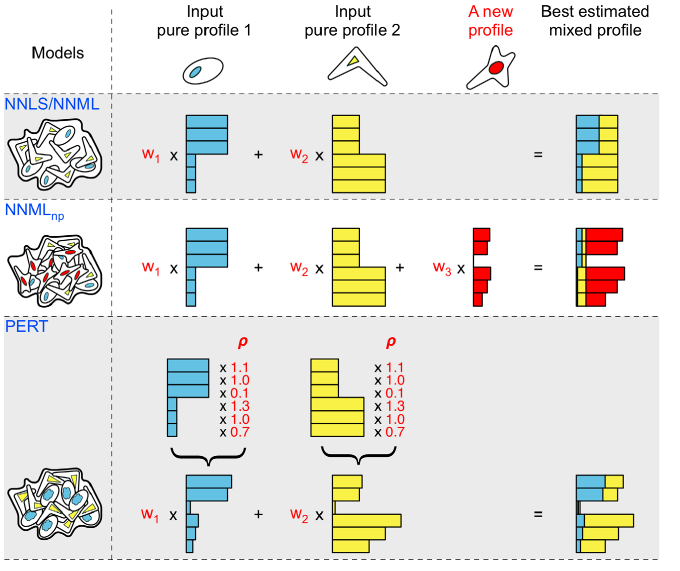
\includegraphics{figures/pert_probalistic_model.PNG}
%\caption{The main four assumptions of the probalistic models benchmarked
%by PERT approach}
%\end{figure}

TEMT (Transcript Estimation from Mixed Tissue samples)
\autocite{li_xie13} is also a
probabilistic model used for deconvolving mixture samples, originally
designed to infer the proportion of transcripts from a two-component
mixture (for instance, setting apart tumoral and normal immune cells)
but that can easily extended to deconvolve any number of cell
populations, provided a purified expression profile is available.
Instead of the \acrshort{RNA-Seq} counts generally required for most of the
deconvolution analyses (an integer number for each sampled transcript),
the read sequence is required, as well as length and sequence of the
transcripts. Actually, one read can be asserted to multiple transcripts
due to alternative splicing (a single DNA coding sequence for a gene can
produce distinct mature RNA transcripts, encoding possibly for proteins
with various functions) or similarity of the sequence, with a higher
proximity among homologous genes. One of the main objective of TEMT,
making it applicable for normalization of purified samples, is removing
non-biological variability. Indeed, only a part of the differences
observed in the number of counts between the transcripts is explained
biologically (the nature of the cells sampled, for instance, Lymphocytes
B express more IL4R than the other cell populations, or the phenotypical
status), but another part is associated to technical artefact.
Accordingly, for two genes expressed in the same proportions in a given
cell type, the resulting transcript with the longer sequence (referred
as the \emph{effective length} in the paper) offers more priming sites
to the RNApolymerase to start the transcription, and accordingly the
number of counts associated to it will be artificially superior. Even
trickier, the sequence itself can induce bias, resulting from both
\emph{positional bias} (starting positions of the processed reads are
not uniformly distributed along the sequence, but preferentially
distributed around the ends of the target transcript) computed before
using a binning method and \emph{sequence-specific bias} (the series of
nucleotides in the ends of the sequence, namely the proportions of A, C,
G and T nucleotides), estimated using Markov Chain. To our knowledge,
this is the only partial-based deconvolution method that directly
accounts for technical artefacts in their deconvolving process, as other
methods generally consider that input data has already been normalized
for such technical noise (TPM roughly corrects the effective length
bias, but doesn't deal with more specific sequence bias). Finally, the
last perturbation variable comes from the unknown cell population, which
is modelled similarly as in \(\text{NNML}_\text{np}\) algorithm (both
determination of its expression profile and its ratio). Instead of a
Dirichlet prior on the initial distribution of the ratios, a Gamma prior
has been used to initialize individually each ratio. The MLE of the
corresponding log-likelihood of the model is not analytically
computable, hence an online EM algorithm, whose convergence to the true
estimate was shown theoretically in
\autocite{dempster_etal77}, is used to retrieve an unbiased estimate of both the proportions
of a given transcript produced in a cell type, removing the technical
artefact, and the proportions of the cell type itself.
The DAGs describing the generative process of these probabilistic-based deconvolution models are represented in \Cref{fig:probalistic-model}

\begin{figure}
\centering
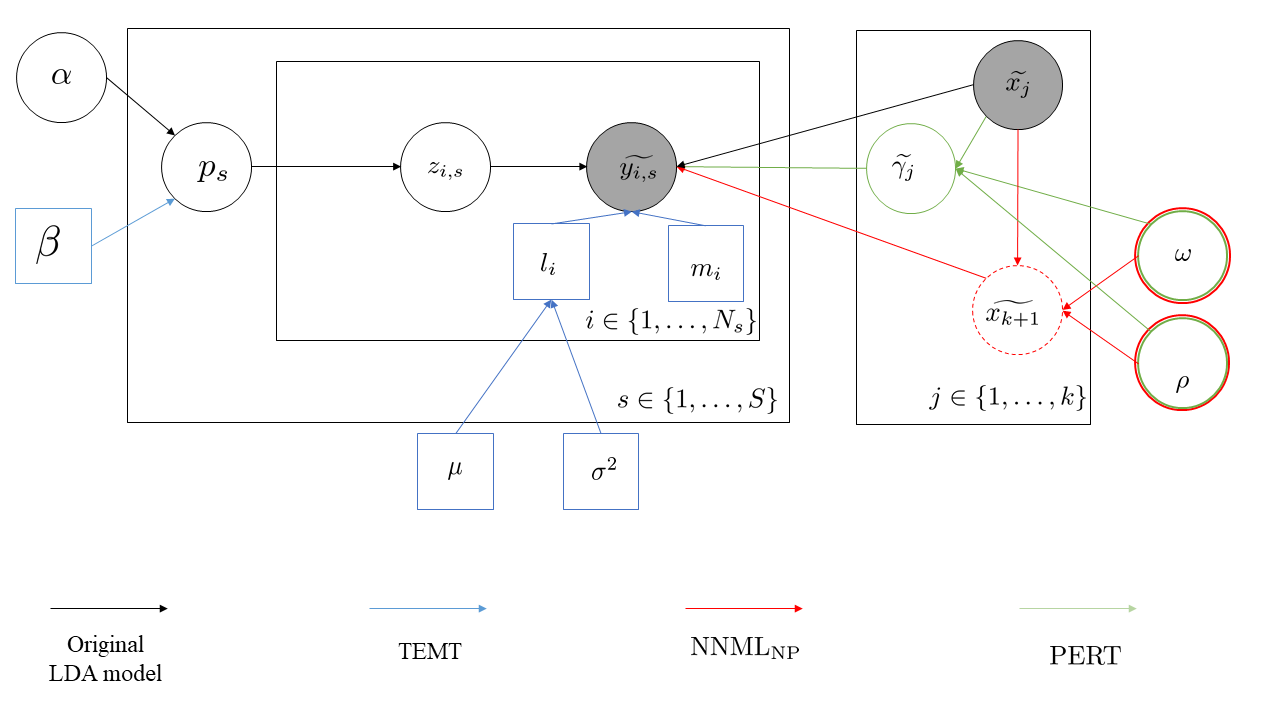
\includegraphics[width=0.5\textwidth]{figures/directed_probalistic_model.png}
\caption{The representative graphical models used to retrieve cell
ratios. More information on
\href{https://revbayes.github.io/tutorials/intro/graph_models.html\#legend}{legende
of a graphical model}}
\label{fig:probalistic-model}
\end{figure}

Lu and colleagues\autocite{lu_etal03} were the first to deconvolve cell proportions in the
transcriptome of yeast cultures in different phases of the cell cycle.
Wang and colleagues estimates immune cell populations (CD4+ and CD8+ T
cells, B and plasma cells and macrophages) in murine mammary gland
samples along with mammary epithelial cells and brown and white adipose
tissues. Following studies focus on the estimation of population cells'
proportions in blood samples, as the diversity of cell populations is
lower than solid tissues. Using transcriptomic profiles of purified cell
populations, these studies were able to estimate either the proportions
of lymphocytes, neutrophils and
monocytes\autocite{gong_etal11}, or 18
different immune cell populations \autocite{abbas_etal09}.


\subsubsection{Estimate cell-specific expression profiles}
\label{estimate-cell-specific-expression-profiles}

The usual method assumes that the gene expression of a cell subset is
uncorrelated to the remaining genes and independent of the
environmental. Hence, we can decompose the problem of retrieving the
cell-specific reference matrix for each gene, considering additionally
fixed expression per cell subset no matter the sample. Hence, the
individual gene expression for each sample is given by {[}{]}, where
this time, the cell specific expression profiles \(x_{ij}\) are the
parameters to estimate. Matricially, this yields for S samples the
following equality: \[
y_{i.}^T=x_{i.}^T \mathbf{P} , \quad y_{i.} \in \mathbb{R}^S, x_{i.} \in \mathbb{R}^{k}, \mathbf{P} \in \mathbb{R}^{k \times S}
\] and the LLS problem to solve is given by: \[
\hat{x_{i.}}_{\text{OLS}} = \arg \min_{\hat{x_{i.}}} \left( ||\hat{x_{i.}} \mathbf{P} - y_{i.}||^2 \right) = \sum_{s=1}^S \left( y_{is} - \sum_{j=1}^k p_{sj}\hat{x_{ij}} \right)
\]

As in CibersortX \autocite{newman_etal19} or the csSM algorithm in
\autocite{shen-orr_etal10}, it may
be possible to add a discrete explanatory variable for which in each
level the cell reference is fixed, but may vary from a condition to
another (for instance, sex or disease state). However, adding this
covariate implies, to keep a determined solution, that the number of
samples in each biological level is superior to the number of cell type
\(k\). Finally, instead of OLS, any linear regression method described
in the previous section can be used to solve the problem (yet, using
robust or SVR-based methods that include a filtering step, here on the
cell types selected, is not really relevant).

\[
x_{ij} \ge 0, \forall j \in \{1, \ldots, k\}
\] \[
Z_1, Z_2 \in \left\{1, \ldots, S \right\}, |Z_1| \ge 2, |Z_2| \ge 2, Z_1 \cap Z_2 =0
\]

\[
\begin{pmatrix}
y_{1, 1} & \ldots & y_{1, |Z_1|} & \ldots & y_{1, |Z_2|}\\
y_{2, 1} & \ldots & y_{2, |Z_1|} & \ldots & y_{1, |Z_2|}\\
y_{3,1} & \ldots & y_{3, |Z_1|} & \ldots & y_{1, |Z_2|}
\end{pmatrix}
=
\begin{pmatrix}
x_{1, 1} &  x_{1, 2}\\
x_{2,1} &  x_{2, 2} \\
x_{3,1} &  x_{3, 2}
\end{pmatrix}
\times
\begin{pmatrix}
p_{1, 1} & \ldots & p_{1,|Z_1|}\\
p_{2,1} & \ldots & p_{2,|Z_1|}
\end{pmatrix}
\]

\[
\forall i \in \left\{ 1, \ldots, 3 \right\}, \forall s \in Z_1
\] \[
y_{3, s} = a_1 y_{2, s} + a_2 y_{2, s}, \forall s \in Z_1, a_1, a_2 \in \mathbb{R}
\]


\subsection{Unsupervised and reference-free deconvolution methods}
\label{unsupervised-and-reference-free-deconvolution-methods}

Complete deconvolution algorithms attempt to simultaneously estimate
both the proportions and the pure expression profile of cell types
\autocite{shen-orr_gaujoux13},
without any additional information than the bulk profile. Such methods
are generally undetermined, thus they require prior information as well
as extra post-processing steps to assign the identified clusters to pure
cell types. Indeed, several optimal solutions can be found, and adding
prior information or constraint, can make the problem identifiable. They
are more sensitive to the amount and quality of data provided.

The first study proposing an algorithm to solve this problem was
published in 2001 by Venet and
colleagues\autocite{venet_etal01}. It
was an iterative method that estimates both \(\boldsymbol{X}\) and
\(\mathbf{P}\) by minimizing the absolute error,
\(|\mathbf{Y} - \boldsymbol{X} \times \mathbf{P}|\) that was applied to
deconvolve colon cancer samples. Interestingly, their method was able to
identify four cell populations, two of which could be identified as
hematopoietic cells and
fibroblasts\autocite{venet_etal01}.
The authors however discuss the limitations of their algorithm, notably
the selection of the appropriate \(k\) number of cell populations.

Repsilber and colleagues extended the method proposed by
\autocite{venet_etal01}, notably by
using a least-square non-negative matrix factorization algorithm,
alleviating one of the hypotheses necessary for the applicability of the
previously-proposed
model\autocite{repsilber_etal10}.
Erkkiläe implemented a Bayesian statistical framework that requires only
the number of distinct cell populations
\(k\)\autocite{erkkila_etal10}.

\autocite{wang_etal15} introduces
the UNDO R package that supplies an unsupervised deconvolution method to
impute both ratios and expression profiles specific to the tumour cells.
It requires however to identify marker genes (MGs) specific to the
tumour population studied. Previously,
\autocite{ahn_etal13} and
\autocite{quon_etal13} also address the
challenging task of purifying biological samples with immune infiltration and contamination in tumoral samples \footnote{Taking into account tumour heterogeneity in cancer genomics increases by several orders the sensitivity and specificity of DGEAs. Nevertheless, it is a challenging task due to the combination of an inter-tumour heterogeneity between different tumour types and an intratumour heterogeneity within a given sample (different tumour subclones). The current studies only addresses the inter-tumour heterogeneity, while in order to study intra-tumour
heterogeneity, either single-cell profiling data or sequences from multiple locations at different time points are needed.}.

Finally, UNDO \autocite{wang_etal15}
and CAM \autocite{wang_etal16} are
unsupervised approaches, allowing novel marker identification. To do so,
the expression matrix is projected in a K-dimensional \emph{polytope}
where each dimension \(K\) corresponds to a cell type present in the
mixture and the vertices to the associated marker genes. The R package
CAMTHC \autocite{chen19} implements the
completely unsupervised CAM algorithm with MDL visualization to help the
users selecting the right number of populations in their mixture. Prior
knowledge on some TMs for a cell type can increase the accuracy and
performance of the algorithm, in a semi-supervised approach where de
novo markers can be added by CAM algorithm. Both versions of this
algorithm are referred and benchmarked in
\autocite{jin_liu21} as CAMfree and
CAMmarker. Additionally, they provide a supervised approach to infer the
cell ratios with a LLS method when the pure signature is available and
NNLS independently for each gene when the cell ratios are provided.


\subsection{Marker-based approaches}
\label{subsec:marker-based-approaches}

In this type of approach, markers and expression profiles specific to a
cell type are required. Ideally, \emph{markers} are thought as genes
entirely specific to one population and robustly expressed in different
biological conditions. But to set apart highly correlated cell types,
this restrictive definition is often relaxed to a gene mostly expressed
in one cell type.

The markers investigated are sometimes proposed on immunology knowledge
Rooney et al. \autocite{rooney_etal15}, but are
most often based on empirical measures of purified (FACS-sorted or
in-vitro cultured) cell populations. The first approach to select marker
genes consisted in finding genes whose average expression value in one
cell type is greater than the expression value across the remaining cell
types \autocite{shoemaker_etal12}.
\autocite{chikina_etal15} extends this approach by assessing whether the difference was
statistically significant (combination of arbitrary fold-change and
\emph{p}-value approaches), by ranking markers based on SNR
(signal-to-noise) ratios \autocite{becht_etal16}, the F-statistic (testing whether adding an additional marker
is relevant in a multiple linear regression model)
\autocite{wang_etal10} or the Gini
index \autocite{zhang_etal17}.
Generally speaking, the methods used to discard genes belong to the
general machine-learning framework of \emph{filtering}, the
pre-processing step that removes irrelevant features before application
of a prediction algorithm
\autocite{guyon_elisseeff03}.

We now define theoretically the basis for using marker genes in
deconvolution problems. Let's consider a cell population \(j\), with
\(G_j \in \{1, \ldots, n\}\) the set of genes expressed uniquely in this
cell population. Then, for any gene from the marker set, we have the
following relation: \[
y_{i, i \in G_j}= \sum_{l=1}^k x_{i, l} \times p_{l} = x_{i, j} p_j, \text{ as } x_{i, l} =0, \forall l \neq j
\] where the existence of a mathematical solution in absence of noise
requires colinearity between the expression of the genes of cell
population \(j\) and the sample's expression of the corresponding genes
in the transcriptome \(y_{i, i \in G_j}\). This implies that for any
gene belonging to the market set, we have the following relationship: \[
p_{j}=\frac{y_i}{x_{i, j}}, \quad \forall i \in {G_j}
\] or, alternatively, that any gene expression is correlated to the
remaining genes of the market set.

This relationship can be generalized to \(S\) samples and to the \(k\)
cell populations of interest, with the genes expressed in the population
cells represented by the following \emph{block diagonal matrix} \[
\begin{pmatrix}
y_{G_1, 1} & \ldots & y_{G_1, S}\\
y_{G_2, 1} & \ldots & y_{G_2, S}\\
\vdots & \ddots & \vdots \\
y_{G_nn,1} & \ldots & y_{G_n, S}
\end{pmatrix}
=
\begin{pmatrix}
x_{G_1, 1}  &\ldots & 0\\
0 & x_{G_2, 2}   & 0\\
\vdots & \ddots & \vdots\\
0 & \ldots & x_{G_k, k}
\end{pmatrix}
\times
\begin{pmatrix}
p_{1, 1} & \ldots & p_{1, S}\\
p_{2, 1} & \ldots & p_{2, S}\\
\vdots & \ddots & \vdots \\
p_{k,1} & \ldots & p_{k, S}
\end{pmatrix}
\] with \(x_{G_j, j}\) the expression of markers genes uniquely
expressed in population \(j\). We generally set apart unsupervised
methods where neither the reference signature nor the cell ratios are
provided from supervised methods where one of these elements is known.
But both methods assume that markers specifically associated to a cell
population exist. Furthermore, there's no deconvolution technics going
down to the transcript level, while alternative transcript expression
may help in setting apart close cell types.


%\subsubsection{Infer ratios}
%\label{infer-ratios}
%
%However, in real datasets, the linear relationship assumption is broken
%by the presence of a random noise:
%\(y_{j}=x_{j}\times p_{j} + \epsilon_j, \quad \forall j \in G_j\).
%Historically, marker-based deconvolution methods rely on the
%identification of one \emph{strong} marker with a gene expression
%specific to only one cell population Clarke, Seo, and Clarke
%\autocite{clarke_etal10}. \autocite{gosink_etal07} assumed that the minimal expression ratio between the
%mixture and the reference signature \(\frac{y_{j}}{x_{j}}\) can be used
%as a proxy, up to a multiplicative constant, of the population
%associated to gene \(j\). It was originally designed to estimate the
%tumoral proportion in heterogeneous samples, and may not well-adjusted
%when retrieving ratios of several cell types. Additionally, it assumes
%that the noise effect is minimal and that a gene is uniquely expressed
%in the population of interest. An extension of this work is proposed in
%\autocite{clarke_etal10}
%that use the same algorithm but applies a specific log transformation.
%This may reduce the noise impact associated to small ratio values and a
%general underestimation of the true proportion. However, as suggested in
%several benchmarks Fa et al. \autocite{fa_etal20},
%log-transformation generally has a negative impact on the performance.
%
%More recent studies alleviate the null-expression condition, identifying
%\emph{weak} markers over-expressed in a given cell population but with
%possibly non-null expression levels in the others. They also focus on
%identifying not only one specific gene per cell type, but a collection
%of them, which is then either aggregated into an abundance score
%(MCPcounter, Becht et al., 2016) or an enrichment score (xCell, Aran et
%al., 2017).
%
%The abundance score is computed by averaging the expression ratios of
%the bulk mixture and the reference profile over the set of markers Becht
%et al. \autocite{becht_etal16}, and may be used as
%an approximate estimate of the ratios of cell subsets:
%
%\[
%\hat{p_{j}}=\sum_{i=1}^{n} \frac{y_i}{x_{i, j} |G_j|} \mathbb{1}_{i \in {G_j}}
%\] with \(|G_j|\) the number of marker genes associated to population
%\(j\). In doing so, we compute a more robust abundance score to the
%previous methods taking into account only one marker Clarke, Seo, and
%Clarke \autocite{clarke_etal10}, as the presence of
%an aberrant transcriptomic profile among the set of markers genes may be
%alleviated by the remaining genes. Both methods differ on the filtering
%of cell populations investigated and on the selection of marker genes.
%In \autocite{angelova_etal15}, a
%first cutoff of two FC is applied for the selection of candidate genes
%and then refined by considering only genes highly correlated to each
%other within a marker set. GSEA is then used to identify cell
%populations truly present in the mixture, keeping those enriched in the
%patient sample. In \autocite{becht_etal16}, the selection of TM relies on a compendium of 3 filters: AUC,
%fold change and a tailored fold change that preferentially selects genes
%both highly specific to a cell population and little variable in the
%remaining cell populations. Alternatively to the average of ratios
%proposed above, they propose the MCP-counter score, which is simply the
%log of the geometric mean of the bulk expression of the
%TMs:\(p_{k0} \propto \left(\prod_{j=1}^{n_{k_0}} y_j\right)^{1/k_0}\).
%This score is supposed to be correlated with the true ratio of the
%investigated cell population.
%
%Most of the methods computing an enrichment score (ES) rely on a
%weighted version of the ssGSEA (single-sample gene set enrichment
%analysis) principle, developed first by
%\autocite{subramanian_etal05}
%and \autocite{barbie_etal09} to
%determine whether a gene set was differentially expressed in a given
%biological sample. Let's consider a set of marker candidates for a given
%population \(k_0\) and rank the total number of genes \(n\) of the bulk
%mixture by their normalized expression level (or any other measure of
%the magnitude of their expression). The ES of the marker genes is given
%by: \[
%ES (y_{n_{k_0}}, \overline{y_{n_{k_0}}})=\sup_{i=1}^n \left| P_{y_{n_{k_0}}}(y_i) - P_{\overline{y_{n_{k_0}}}}(y_i) \right|
%\] where
%\(P_{y_{n_{k_0}}}=\sum_{j \le i}^{n_{k_0}} \frac{y_j^{\alpha}}{n_{k_0}}\)
%is the ECDF (empirical cumulative distribution function) of the marker
%genes, possibly weighted by an exponential term, and
%\(P_{\overline{y_{n_{k_0}}}} = \sum_{j \le i}^{n - n_{k_0}} \frac{1}{n - n_{k_0}}\)
%is the ECDF of the ranking of the remaining genes (remember that a
%marker gene is uniquely assigned to a cell population). When
%\(\alpha=0\), this is equivalent to the standard Kolmogorov--Smirnov
%statistic to compare empirical distributions
%\textcolor{red}{cucconi test might be relevant as well}. In all the
%reviewed papers that use this score, the ES was computed with the R
%\emph{gsva} function.
%
%In \autocite{bolen_etal11}, SPEC (Subset Prediction from Enrichment Correlation) is a
%two-step algorithm, aiming at linking a change in the gene expression
%with a specific cell population. To do so, enrichment scores (ES) are used as proxys of cell ratios
%for each sample, then the signature input provided by the user is associated to the cell lineage
%with the highest Pearson correlation in terms of ES. SPEC determines
%that the origin of the resistance to the standard treatment of HCV
%patients was the interaction between the myeloid cells and the
%anti-interferon therapy. In
%\autocite{rooney_etal15}, genes with
%at least 2-fold change greater than any observed in remaining cell types
%were selected as TMs. The goal of the study was to link the
%transcriptomic tumoral activity with the cell ratios observed in order
%to uncover mechanisms related to immune tumour resistance.
%\autocite{yoshihara_etal13}
%generates an immune and stromal enrichment score in a tumoral sample,
%averaging them into the E\acrshort{st}IMATE metric. It then uses the Eureqa
%software to determine the best link function associating the tumoral
%purity (proportion of tumoral cells in the sample) to the E\acrshort{st}IMATE
%score. The formula, fitted with the \emph{nls} function from the stats
%package is given by: \[
%\text{tumour purity} = \cos \left(a + b \times \text{E\acrshort{st}IMATE}\right)
%\] An extension of this method, combining metrics from alternative omics
%data, is proposed in \autocite{aran_etal15} paper. It's simply the average of the tumour purity
%estimations from four sources: the E\acrshort{st}IMATE score described above,
%ABSOLUTE (quantify the proportion of cancer cells based on the number
%and location of somatic copy-number mutations), LUMP (correlation
%between the degree of methylation and the tumour proportion) and
%immunehistochemistry image analysis (tumoral cells can be identified
%with specific fluorescent markers). In
%\autocite{senbabaoglu_etal16},
%gene signatures were obtained from biological knowledge, discriminating
%24 distinct cell populations in 19 cancer types. It was shown that
%over-expression of some cell types improved survival (Th17, CD8+ and
%Treg), while Th2 cells increase is associated to a negative prognostic.
%More recently, using a newly designed gene signature
%\autocite{aran_etal17}, xCell
%algorithm claims that it's able to identify up to 64 distinct immune and
%stromal cell types \textcolor{blue}{definition of a stromal cell}, using
%a compendium of 1822 pure human transcriptome. Additionally to a FC
%criterion, oncogenes were pre-filtered in the design of the reference
%matrix, and several signatures could be associated to a given cell type.
%To keep the linear relationship between the computed ES and the true
%cell ratio across several data sources, calibration was performed by
%means of a power function (only adjusted for average abundant cell
%ratios). Finally, the spillover effect that induces systemic bias in the
%ratios' estimation of highly correlated cell populations is
%counterbalanced by reducing correlated terms of the covariance matrix
%between the cell ratios.
%Finally, TIminer \autocite{tappeiner_etal17} is a freely Docker analytical pipeline. It uses the reference
%matrices provided by\autocite{aran_etal17}, \autocite{angelova_etal15} or
%\autocite{charoentong_etal17} to estimate the enrichment of tumour immune cell types, along
%with neoantigen prediction and tumour immunogenicity to characterize the
%tumoral environment.
%
%\autocite{shoemaker_etal12}
%propose the CTen (cell type enrichment) web-based tool able to
%automatically retrieve highly specific cell's gene expression in
%user-provided pure cell population transcriptome. Enrichment score in
%that paper is the negative log10 of the \emph{p}-value of a a Fisher's
%exact test. A significant \emph{p}-value rejects the null hypothesis of
%independence between the over-expression status of a gene and its
%belonging to a specific cell type TM. In case of independence, we expect
%in average that the proportion of over-expressed genes within the marker
%set and the non-specific genes is equal. This method is not applicable
%when a large number of cell populations are considered or when the set
%of TM is too small. Additionally,
%\autocite{abatangelo_etal09}
%shows that the Fisher's exact test is much worse in detecting small
%enrichments. Another alternative is proposed by the Bioconductor package
%BioQC \autocite{zhang_etal17}, where
%the enrichment of a marker set is asserted comparing the median
%expression of the TMs with the median expression of the bulk mixture,
%asserted with the non-parametric \emph{Wilcoxon-Mann-Whitney test}.
%
%Last but not least, both abundance and enrichment methods do not return
%the exact relative proportions of cell populations in the bulk sample,
%but only a score correlated to it. While most studies assume that
%there's a linear relationship between the score and the true ratio,
%\autocite{aran_etal17} is the
%only marker-based method in our review that attempts with numerical
%simulations to clearly retrieve the parameters of a link function, which
%reveals non linear (here, a power function). Hence, as opposed to whole
%transcriptome based methods, marker-based technics are more dedicated to
%inter-sample comparisons than intra-sample comparison.
%
%
%\subsubsection{Infer reference profiles}
%\label{infer-reference-profiles}
%
%\autocite{kuhn_etal11} and \autocite{kuhn_etal12} design the
%Population-Specific Expression Analysis (PSEA), the only method of our
%review using FACS data to estimate cell type-specific expression levels.
%Their method includes an intersection term to include non accounted cell
%types in the bulk expression, however they assume that within a
%biological group, the specific expression of a given cell type is the
%same for all individuals. It has been designed to identify the
%correlation between expression changes in astrocytes and Alzheimer's
%disease progression. More generally, their design is more adjusted to
%perform differential analyses testing whether the specific expression of
%a gene within a cell type is differentially expressed in relation with a
%biological condition. \autocite{reinartz_etal16} paper supplies as well a method dedicated to infer cell
%type specific expression, but it requires pure reference signatures of
%the cell types of interest, with small overlap between their
%transcriptomic expression. Additionally, the cell ratios and corrected
%pure cell types expression in a mixture are systematically biased, with
%an underestimation of the infiltrate cell type, or even worse, the
%adjustment performed is likely to be confounded with the natural
%variability of the transcriptomic expression.
%
%\todo{look at EPICabsolute and TIMERtumor}
%
%
%\subsubsection{Infer ratios and pure transcriptomic expression}
\label{infer-ratios-and-pure-transcriptomic-expression}

One of the first unsupervised technics, requiring only a set of specific
TM for a given cell type, is the Digital Sorting Algorithm (DSA) Zhong
et al. \autocite{zhong_etal13}{]}. First, we
hypothesise that the pure expression of a TM can be summed up by its
mean, yielding the following pure reference matrix:

\begin{equation}
\widetilde{\boldsymbol{X}_{1:k, 1:k}}
=
\begin{pmatrix}
\overline{x_{n_1, 1}}  &\ldots & 0\\
0 & \overline{x_{n_2, 2}}   & 0\\
\vdots & \ddots & \vdots\\
0 & \ldots & \overline{x_{n_k, k}}
\end{pmatrix}
\label{eq:marker-based}
\end{equation}

where \(\overline{x_{n_j, j}}\) is the average expression of the TM
set of population \(j\). Then, using \Cref{eq:marker-based} and simplex-unit constraint, listed in \Cref{eq:simplex-constraint}, we obtained the
following system of linear equations, with \(k\) unknown pure aggregated
TMs: \[
\begin{cases}
\sum_{j=1}^k \frac{y_j1}{\overline{x_{n_j, j}}}&=1\\
& \vdots \\
\sum_{j=1}^k \frac{y_jS}{\overline{x_{n_j, j}}}&=1
\end{cases}
\] Provided that the number of samples exceeds the number of cell types
(\(k < S\)), we can solve the system, and use the corresponding
aggregated matrix \(\widetilde{\boldsymbol{X}_{1:k, 1:k}}\) to retrieve the cell type ratio matrix with
classic linear regression. Once done, the estimated cell ratios are used
to retrieve the distinct pure expression profile, using
quadratic programming with bounded constraint for the expression.
CellCODE \autocite{chikina_etal15} models the proportion of the cell type of interest as a
surrogate variable, retrieved as the first right singular vector
(denoted as \emph{eigengene}, contributing the most to the variability
observed in the considered TM set). To reduce the searching space, the
estimation of the surrogate proportion variable (SPV) is restrained to
an user set of TMs specific to the cell population of interest.
Additionally, to account for the biological effect, it's possible to
integrate the design experiment in the study, although limited to a
single explanatory variable. The main purpose of this study is then to
integrate the estimated ratios to demingle the effect resulting truly
from a dysregulated expression of the TM to the effect of a modification
in the cell population. Their study notably shows that using this
process increases the sensitivity of their differential analyses.
However, we should note that the additional variability captured by the
surrogate variable may not be explained by a change in cell population
composition but rather from a technical effect or an uncaptured
biological condition \autocite{venet_etal01}.




\subsection{Alternative omic data types used for the deconvolution}
\label{alternative-omic-data-types-used-for-the-deconvolution}

Recently, epigenomics has been increasingly used for the deconvolution
problem. EpiDISH
\autocite{teschendorff_etal17} and methyICC \autocite{hicks_irizarry19} infers cell-type composition using DNA methylation data
and a reference profile of the CpG sites. Indeed, the degree of
methylation of the CpG sites of the DNA sequence is highly correlated to
the level of the gene expression and highly specific for a given gene to
the cell population. TOA\acrshort{st} \autocite{li_etal19}, BayesCCE \autocite{rahmani_etal18}, Edec \autocite{onuchic_etal16}, RefFreeEwas
\autocite{houseman_etal16} and MeDeCom \autocite{lutsik_etal17}
retrieve both the cell ratios and methylome reference profiles in a
completely unsupervised manner. Most of these methods use the same NNMF
algorithm, but set apart in the details of the implementation of the
method. For instance, RefFreeEwas initiates the population clusters
using hierarchical clustering, while Edec and Medecom use random
initialisation. Finally, Aran et al.~(2015) built a score, the Consensus
measurement of Purity Estimation, to evaluate the tumour purity in the
sample, combining transcriptomic, somatic copy number, methylation and
immunohistochemistry data.

However, as Teschendorff and Zheng (2017) pointed out, there's currently
no benchmark comparing the cell ratios retrieved from either
expression-based or DNA methylation-based, neither any attempt of
multi-omic integration data to solve the deconvolution problem.


\section{Feature selection}
\label{sec:feature-selection}

\todo{to be linked with the RNA-Seq pipeline}

Generally, following steps are considered for solving bulk mixture problem:

\begin{itemize}

\item
  creation of a reference gene signature profile when not provided
\item
  mixture model solved using svr or linear regression
\item
  statistic tests evaluating for each cell ratio estimation if it's
  significantly different from 0
\item
  (if provided) comparison with reference cell ratio measures, for
  instance using flow cytometry for instance
\end{itemize}

\todo{un-normalized RNA-seq is more accurately described by a negative binomial distribution// methods that do not rely on data normality, like LDA models, cf finotello in review section.}

The definition of a \emph{transcriptomic marker} for a cell population
is unclear and varies from one study to the other. In most partial
deconvolution approaches, the used markers of cell populations are
simply the differentially expressed genes.

Cell-types matrices were obtained by differential expression analysis.
Differentiation is asserted via an unequal two-sided variance t-test,
and a global \(q-value\) is computed (FDR process, with an extra step of
estimation of \(H_0\) distribution of p-values). For the estimation of
the total number of distinct genes to be used \(n\), \emph{condition
number} was applied to assert stability and robustness of cell
signatures with noise (especially presence of other cell types or
specifific phenotypic conditions), keeping the one with the lowest
condition number obtained with \(n=547\). With CIBERSORT, such a process
is done using \emph{kappa} function.

To derive a signature from that matrix, an extra-step of filtering is
required, to remove irrelevant feature (in our case, remove genes that
are not useful to discriminate several cell types). This enables a
faster computation (removal of genes with uniform expression, no matter
the cell type, such as those implied in metabolic processes) and a
greater signal-to-noise ratio, by keeping the most discriminatory genes
in terms of expression.

For LM22, either RMA or MAS5 normalization was performed, with HUGO
annotation, for Affymetrix chips. Illumina BeadChip was analyzed using
background correction of limma package \emph{normexp}. All microarray
studies were also processed a quantile normalization step.

An extra-step specific to LM22 generation consisting in a two-step
filtering was performed:

\begin{itemize}
\item
  Exclude genes presenting a too-much enriched expression in
  non-hematopoietic cell types. To that purpose, using enrichment scores
  from Gene enrichment profiler, they exclude all genes whose expression
  score was found higher at a threshold of \(5\%\) in non-hematopoietic
  cells or tissues (that's say not linked with blood cells or blood cell
  formation). We thus remove the ones not specific to the cell types we
  want to describe.
\item
  Second step is removing all genes with a heavy expression (superior in
  log scale to 7) in cell lines profiled in CCLE.
\end{itemize}


Ultimately, although \acrfull{scrna} (see \Cref{subsec:sc-rnaseq}) and \acrfull{st} (see \Cref{subsec:st}) had revolutionised the transcriptomics, we anticipate continuous uphold for the integration of deconvolution techniques as a complementary tool, since both methods are far from reaching the sensitivity and affordability of more traditional \acrshort{ngs} methods. Integration of deconvolution methods enhance the precision and robustness of downstream analysis, notably for identifying in a holistic framework key drivers involved in cell type-specific differential gene expression.


\section{Useful links: Benchmark of deconvolution methods in scientific literature}

Several benchmarks have been developed recently to compare the
performances of numerical deconvolution methods in relation with the
cell type sampled (presence of unknown or highly correlated cell types,
rare populations poorly represented in the transcriptomic compendium, )
(\autocite{sturm_etal19}), the
pre-processing protocol before applying the deconvolution algorithm
itself (\autocite{fa_etal20}) or the
quality of the mixture sample itself (noise structure and magnitude,
number of cell populations to identify, presence of unknown cell types)
\autocite{jin_liu21}.

\begin{enumerate}
\def\labelenumi{\arabic{enumi}.}

\item
  \autocite{fa_etal20} benchmarks several
  combinations of scaling/normalization and transformation technics with
  deconvolution algorithms. \emph{Data normalization} covers all
  techniques to make samples' distribution comparable, including various
  scaling methods (min-max, \emph{z}-score, row or column-wise) and
  methods dedicated to a specific technology, such as \emph{TPM} or
  \emph{FPKM} with RNA data. They may also correct technical artefacts,
  for instance, in \acrshort{RNA-Seq} data, lowly expressed genes are associated
  with a higher variability. The library size (the total number of
  counts measured in a given sample) may also differ between the
  samples. Data scaling approaches transform the data into bounded
  intervals. \emph{Data transformation} refers to the \emph{link
  function} applied on data, such that the assumptions on the
  distribution apply. \emph{Linear transformation} is simply the
  identity link function, with no transformation of the data. Another
  common transformation in transcriptomics data, especially for
  \emph{DGEA} analyses, is the \emph{log2} transformation to make the
  transcripts distribution Gaussian. All pre-processing methods and
  algorithms used to retrieve cell ratios in
  \autocite{fa_etal20} benchmark are
  summed up in the following picture:
\end{enumerate}

\begin{figure}
\centering
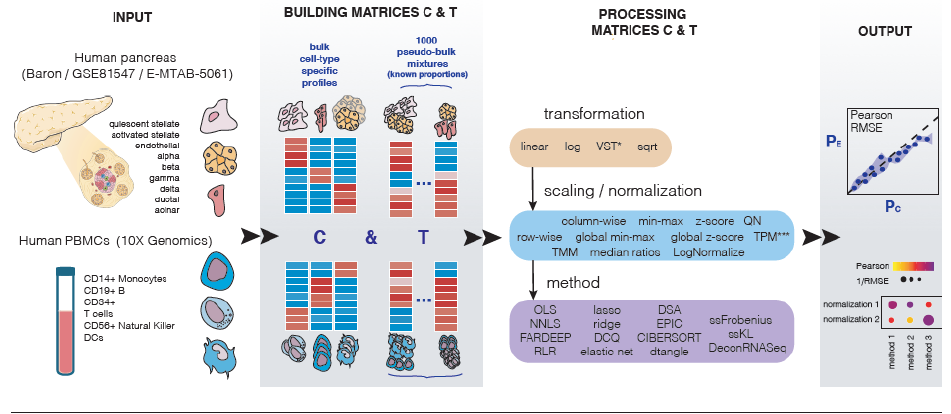
\includegraphics[width=0.9\textwidth]{figures/benchmark_GEP_schema.PNG}
\caption{Benchmark GEP technics}
\end{figure}

Both measures, independently on the platform (\acrshort{RNA-Seq} or microarray) used
or the tissue sampled, concludes that the log-normalization is
underachieving, with best results yield without any data transformation.
\emph{Scaling}, by smoothing extreme values, decreases the overall
performance, while \emph{normalization} within samples, for instance
batch correction of a technical artefact, have little impact on the
results (at the exception of row scaling, column min-max, column z-score
or quantile normalization that yield sub-optimal performances).
Specifically, Jin and Liu \autocite{jin_liu21}
shows that the best performances were reached when both the reference
signature and the bulk matrix of the measured transcripts were applied
the same normalization protocol. Specifically, quantification unit
technics (CPM, TPM, \ldots) that normalize \acrshort{RNA-Seq} data by library sizes,
with TPM being the most commonly used technics, present the best
performances overall.

Pre-filtering genes having the best discriminating power (ones with the
highest expression difference within cell type) tends to improve the
results. More precisely, the highest reproducibility of deconvolution
methods is reached by optimizing the \emph{condition number} (CN) of the
designed reference profile (A. Newman et al.
\autocite{newman_etal15}). Benchmarks on real
datasets seem to show that it was minimal with a moderate number of
genes selected. The CN is given by the following equation,
\(||\boldsymbol{X}|| \times ||\boldsymbol{X}^{-1}||\), with \(||\quad||\) the
Frobenius norm, and can be interpreted as an upper bound on the
precision of the obtained solution. With a CN of 1 (best case), the
accuracy of the solution is of the same order as the intrinsic
variability of the data. The lowest CN (1) is obtained for an orthogonal
matrix, implying in our deconvolution context that the transcriptomic
expression is independent between the cell populations.

The expression profiles are platform-specific, which might result in
markers not being captured by all platforms and in expression levels
depending on the choice of the platform. To counterbalance technical
artefact, CibersortX \autocite{newman_etal19} supplied a batch-correction effect using the Combat
method. Generally, Cibersort, CibersortX and MuSiC are the least
impacted by the choice of normalization protocol. Additionally,
single-cell deconvolution methods in which the reference signature
proceeds explicitly from  \acrshort{scrna} data do not show significant
improvement over more classical methods based on bulk-deconvolution
methods.

\begin{enumerate}
\def\labelenumi{\arabic{enumi}.}
\setcounter{enumi}{2}

\item
  Most of the methods are highly sensitive to the absence of a cell
  population in the reference signature when it's really present in the
  bulk mixture. Hence, \autocite{sturm_etal19} concludes that the best estimates are reached when the
  reference profile is representative of the true bulk cell population.
  Interestingly, the highest deviations occur in absence of
  significantly correlated cell types (\emph{multicollinearity} refers
  to situations where more than two cell types are strongly correlated).
  For instance, the performance in terms of correlation and mean
  absolute deviation (mAD) is highly decreased when mDC (myeloid
  dentritic cells) are present in the mixture, due to their proximal
  expression with monocytes. Especially, when the proportion of a given
  cell population is higher than expected, occurring especially when
  related cell types are not referenced in the signature,
  \autocite{sturm_etal19} mentions it
  as \emph{spillover effects}. They tend to have a greater impact on
  marker-based approaches. \emph{Background prediction} tackles with the
  opposite problem, when a cell ratio is statistically different from zero while it was not present in the mixture. It may explain why most of the numerical deconvolution methods are
  biased, tending to over or underestimate most of the cell types in the
  sample. Additionally, marker methods require an enough number of distinct
  genes (5-10) to identify unequivocally a cell population
  \autocite{ahn_etal13}, especially to
  deal with possible outliers. This issue is exacerbated when some of
  the genes used in the reference signature are both expressed in
  low-abundance and more abundant cell subset (\emph{signal dilution
  effect} \autocite{shen-orr_gaujoux13}. More precisely, \autocite{fa_etal20} suggests that removing a cell type that is uncorrelated
  to all other cell types remaining in the reference matrix tends to
  biased estimates of the ratios of all other cell types while removing
  a cell type that is strongly positively correlated with cell types
  still present in the reference matrix leads to biased estimates
  specifically for them. CibersortX, Cibersort and MuSiC are the least
  sensitive algorithms to the presence of highly-correlated cell types
  or to the presence of rare cell types in the
  mixture\autocite{jin_liu21}
  Additionally, some rare cell types, some being recently discovered,
  may not have been profiled yet, leading to systematic bias in the
  estimation of the cell ratios. This is especially an acute problem
  with tumoral profiles due to the unique patterns of mutations and the
  possibility diversity of subclonal populations. Methods specifically
  tailored to deal with infiltration of cell populations of unknown
  transcriptomic expression, such as TIMERtumor
  \autocite{li_etal16} or EPICabsolute
  \autocite{racle_etal17}, present the
  least biased cell ratio estimations in presence of unknown tumoral
  content.
\end{enumerate}

The results are really dependent on the \emph{phenotypic and tropic
condition}, and the discrepancy between the phenotype (age, gender,
disease status\ldots) of the references samples and the samples in which
the deconvolution is performed could bias the estimated cell ratios.
Additionally, even with similar tissues, individual singularities such
as cellular \emph{heterotypic} contamination (for instance, infiltrates
of tumoral cells), disease-induced or microenvironment dysregulation can
significantly modify the native transcriptomic profiles of the cell
populations compared to healthy tissues. Finally, most reference
profiles provided by deconvolution methods lack samples to capture the
variability of intracellular expression. For instance, the mean
expression of some of the cell types in the LM22 signature of Cibersort
\autocite{newman_etal15} was
estimated from three distinct samples.

In order to get closer from the true biological dynamics, deconvolution
methods could integrate the dynamics of cells types, as in each sample,
different phases of the cell cycle, characterized by varying levels of
transcriptomics expression activity, coexist. While in cultured cells,
the cell cycle can be synchronized by chemical arrest or nutrient
starvation \autocite{bar-joseph_etal08}, this is not possible when alive tissue samples are profiled.

While most methods assume that the expression of individual markers is
independent of the population ratios, Kuhn et al.
\autocite{kuhn_etal11} show that \emph{paracrine}
(proximal cellular communication altering only the behaviour of
neighbouring cells) signalling effects induce high cross-product values
across transcripts.

\begin{enumerate}
\def\labelenumi{\arabic{enumi}.}
\setcounter{enumi}{3}

\item
  Penalized regression approaches including Lasso, ridge, elastic net
  regression and DCQ performed in average slightly worse compared to the
  other deconvolution methods. Quadratic programming (DeconRNASeq),
  Digital Sorting Algorithm (DSA) and the semi-supervised approaches
  ssKL and ssFrobenius (using only sets of marker genes, in contrast to
  the supervised counterparts which use a reference matrix with
  expression values for the markers) showed the poorest performances. As
  against, regression-based (least-squares, support-vector (CIBERSORT)
  and robust regression (RLR, FARDEEP) approaches) bulk deconvolution
  methods, coupled with single-cell data, have the best performances.
\end{enumerate}


%\section{Applications of numerical deconvolution methods}


\label{applications-of-numerical-deconvolution-methods}


\subsection{Differential analysis}
\label{differential-analysis}

\autocite{elloumi_etal11} is one of
the first authors highlighting the loss of power and the risk of wrongly
identifying transcripts expression as prognostic markers of a disease,
when the biological effect is confounded with a change in cell
composition. Indeed, it shows with numerical simulations that ignoring
the contamination of normal cells within tumour cells deflates the power
of detecting breast genomic predictors.

The algorithm \emph{contamDE} \autocite{shen_etal16} offers to model each gene expression in the tumoral
mixture as the contribution of pure tumoral and normal cell population
weighted by their proportion in the sample. The total number of counts
retrieved from \acrshort{RNA-Seq} experiment is hence modelled by the sum of two
negative binomials (NBs), a commonly used probability distribution in
such study. The specificity of their model is to integrate directly the
effect of cell proportion as well as the normalization factor (when the
depth sequence is heterogeneous along with the sample) in the negative
distribution: \[
Y_{ij}^{\text{pure}} \sim \text{NB} (\kappa_j \mu_i, \phi_i) \text{ and } Y_{ij}^{\text{mixture}} \sim \text{NB} (\kappa_j^{'} \left( \mu_i + \omega_j \delta_i\right) , \phi_i)
\] where \(Y_{ij}^{\text{pure}}\) is the number of reads of gene \(i\)
for the \(j^{th}\) sample, \(Y_{ij}^{\text{mixture}}\) the number of
reads in the mixture sample, accounting for both the contribution of
tumoral and normal cells, \(\kappa_j\) and \(\kappa_j^{'}\) are
normalization factors and \(\delta_i = \mu_i' - \mu_i\) the true mean
expression difference between tumours and normal cells. Relevant
prognostic markers are those for which this difference, \(\delta_i\), is
not null. It's worth noted that this distribution is different from the
following mixture model, 
\[
Y_{ij}^{\text{mixture}} \sim (1 - \omega_j) \text{NB} (\kappa_j \mu_i, \phi_i) + \omega_j \text{NB} (\kappa_j^{'} \left( \mu_i + \delta_i\right) , \phi_i)
\] 
that could be expected to simulate the two counts sources, the
purpose being to ease the difficulty of deriving confidence intervals of
DE genes. They also include another model in their analysis, adding an
additional fix effect, to account for possible correlation when the pure
sample and the mixture sample proceed from the same source. Finally, the
unknown parameters of the model (mean of the genes distribution and cell
proportion) are estimated with an iterative method and the final
\emph{p}-values are derived using a likelihood ratio test. However, to
make the problem identifiable, as the pure expression of tumoral cells
is unknown, an additional constraint on the ratios must be set, which
lead to systematic bias toward 1 between the estimated and the true fold
change (no bias in pure samples).

\todo{micro-environment application, \url{https://www.sciencedirect.com/science/article/pii/S0945053X23000811}}
%\section{Biological application}
%\subsection{Tumoral micro-environment}
%
%Cancer is one of the first causes of mortality in developed countries
%(first cause in France, second factor in the USA). In the meantime, it
%remains challenging to develop treatments adjusted to the wide diversity
%taken by cancer forms. Additionally, most of the existing treatments do
%not adjust to the specificity of the tumoral environment, and present
%numerous side-effects.
%
%However, recently, a newly developed treatment, cancer immunotherapy,
%using \emph{immune checkpoint blockers}, reveals highly successful in
%curing tumours that were resistant to standard drug therapies. But the
%tumour microenvironment (TME) {``Low-{Heterogeneity Melanomas Are More
%Immunogenic} and {Less Aggressive}''}
%\autocite{LowHeterogeneity19} is a complex network
%of an interwoven mixture of malignant cells and healthy cells, including
%immune cells and fibroblasts, that intercommunicate. And immunotherapy
%requires a comprehensive molecular and cellular characterization of the
%tumoral environment to elucidate the complex interactions intervening in
%the TME and develop therapies adjusted to any type of cancer form
%\autocite{finotello_trajanoski18}. Indeed, the mechanism of immuno-resistance remains largely
%unexplained, with cold tumours having a poor immunogenic activity with
%low infiltration of T cells and small response to immune checkpoint
%inhibitor therapy (as opposed to hot tumours).
%
%Next-generation sequencing (NGS) as well as novel technologies such as
%single-cell RNA sequencing ( \acrshort{scrna}) and mass cytometry by time of
%flight (CyTOF) provide large data sets that give relevant cues for the
%development of innovative treatments. Accordingly, storing, analysing
%and vizualizing the large and heterogeneous amount of data returned by
%NGS require an intensive research on developing adapted computational
%algorithms.
%
%The \emph{cancer-immunity cycle} \autocite{chen_mellman13}
%consists in the chronological description and evolution of the
%interactions between immune and tumour cells. Complete characterization
%of the tumoral landscape includes thus to retrieve information on
%neoantigens, immune contexture, the tumour microenvironment (TME), and
%global environmental factors.
%
%Cytotoxic CD8+ T cells are responsible for most of the anti-cancer
%response. First, it requires phagocytosis of a newly exogenous foreign
%protein, generated by the gene mutations or rearrangements occurring in
%tumoral cells, by an APC (antigen-presenting cell), generally a DC
%(dentritic cell). Then, proteolytic enzymes cleave the protein into
%smaller peptides that are transported to the cell surface via newly
%synthesized MHC class II molecules from the endoplasmic reticulum. Next,
%priming and activation of naive CD8 T cells occurs in lymph nodes where
%the antigen is presented by the MHC class II complex of an APC together
%with co-stimulatory signals. Finally, after clonal expansion and
%proliferation of the activated T cells, the anticancer immune response
%is exerted through recognition of an endogenous peptide bound to MHC
%(major histocompatibility complex) class I of tumoral cells (the
%so-called peptide-HLA complex) by the variable part of the TCR chain of
%a TCD8 cell and secretion of molecules such as granzyme B (GZMB) and
%interferon-\(\gamma\) (IFN\(\gamma\)) that lyse the cell membrane. It's
%worth noted that both MHC classes are encoded by distinct HLA gene
%complexes. Interestingly, the proteasomes of any cell type generate
%peptides from all proteins present within the cell that are presented to
%the surface, but their recognition as \emph{non-self} requires
%necessarily that the corresponding TCD8 \emph{clonotype} (populations of
%T cells that carry identical TCRs) has first been activated and
%amplified by an APC. Immune checkpoint blockers are monoclonal
%antibodies (specific to one antigen only) targeting receptors present on
%either tumour or immune cells that can boost the inflammatory response
%against cancer cells, generally by their antagonistic action on the
%inhibitory mechanisms developed by tumoral cells. The in silico
%prediction of the \emph{immunogenicity} (ability of a molecule to
%provoke an immune response) of neoantigens are at the core development
%of personalized cancer vaccination and immunotherapy. It requires three
%steps: first, identification of somatic mutations from paired tumour and
%normal tissue; second, genotyping of the patient's HLA genes and, third,
%prediction of peptides binding to the patient's HLA molecules. Two
%prognostic signs associated to a higher immunogenecity include the
%stability of the pHLA complex altogether with the \emph{avidity} (T
%cells with high functional avidity respond to low antigen amounts) of
%the TCR receptor, especially the CDR3 sequence, region of the variable
%chain that binds to the eiptope of the antigen Rasmussen et al.
%\autocite{rasmussen_etal16}, and the foreignness of
%the neoantigen \autocite{blank_etal16}
%(a never recognized peptide is more likely to induce a higher reaction).
%
%\begin{figure}
%\centering
%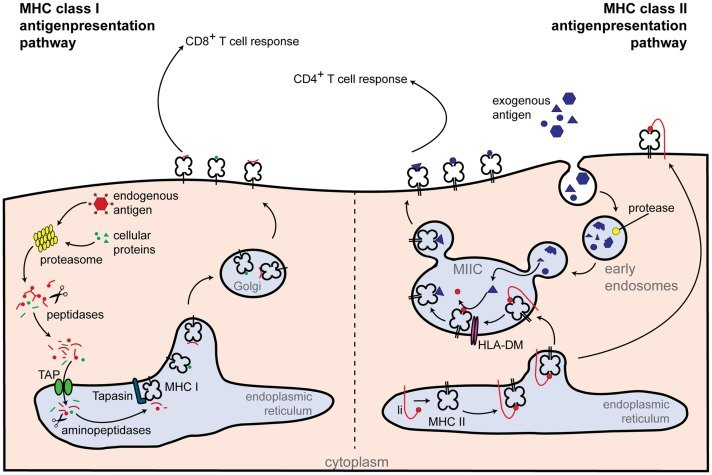
\includegraphics{figures/Classical-routes-of-antigen-presentation-by-MHC-class-I-and-II-molecules-Class-I-antigen.png}
%\caption{Description of the differences between the mechanisms of
%antigen presentation by- MHC class I and II molecules
%\autocite{neerincx_etal13}}
%\end{figure}
%
%The immune context describes the composition (ratio of effectors and
%suppressors cells of the immune reaction), the localisation of
%infiltrating (infiltrated: immune inflamed phenotype, confined at the
%tumour margins: the immune excluded phenotype or absent from the tumour
%mass: immune desert phenotype) and their state of activation. Indeed, by
%exerting pro- and anti-tumorigenic actions, tumour-infiltrating immune
%cells can profoundly influence tumour progression, as well as the
%success of anti-cancer therapies Galluzzi et al.
%\autocite{galluzzi_etal18}. For instance, cytotoxic
%CD8+ T cells can specifically recognize and kill tumour cells bearing
%neoantigens \autocite{chen_mellman13}, while regulatory T cells, by their immuno-suppressive
%functions, can enforce immune escape
%\autocite{finotello_trajanoski17}. Understanding the interaction and communication among distinct
%cell populations is also crucial to help understanding the evolution of
%the tumoral population. Proteomics and secretome (what is released into
%the extracellular space) data can help deciphering the various cell
%communication pathways, including chemokines or cytokines with their
%coupled receptor or immune checkpoint ligand--receptor pairs
%\autocite{rieckmann_etal17}.
%
%The spatial range of cytokine-mediated communication is also key to
%unveil the complex network of interactions between the cell populations,
%with three modes of cell signalling: \emph{autocrine signalling}, in
%which secreted cytokines are trapped by receptors from the same cell;
%paracrine signalling, in which secreted cytokines are trapped from
%receptors of cells belonging to the same tissue; and endocrine
%signalling, in which secreted cytokines are generally carried by blood
%vessels to distant remote tissues
%\autocite{thurley_etal15}. Analysing
%the ligand--receptor interactions helps recently to elucidate the
%mechanism of action of a ligand secreted by epithelial cell on a
%receptor present in cancer-associated fibroblasts of the ovarian cancer
%\autocite{yeung_etal19}.
%
%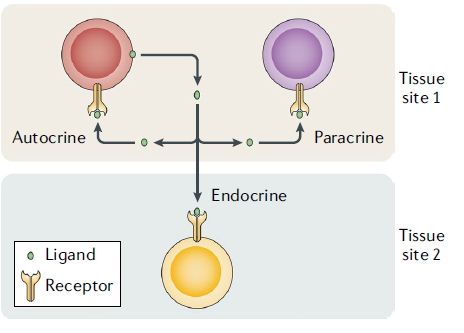
\includegraphics{figures/cell-cell_communication.PNG}
%
%The TME encompasses, in addition to tumoral and immune cells, other
%healthy non-immune cells, such as epithelial and endothelial cells,
%mesenchymal stem cells and cancer-associated fibroblasts (CAFs).
%Notably, CAFs release various tumour-promoting cytokines and chemokines,
%hence favouring tumour growth, angiogenesis (and so risk of the
%development of metastatis) and immunosuppression. Indirectly, pericytes
%play a role in the development of tumoral clones, by regulating the
%contracton of the blood vessels.
%
%Global environmental factors, such as angiogenesis, tumour-promoting
%inflammation and immunological competence of the patient, such as
%infection state or immuno-mediators drugs have a strong impact on the
%composition of the TME. Additionally, commensal microbes from the gut
%microbiota can modulate the antitumour immunity.
%
%
%
%Major challenges remain to understand this intricate system, including
%the comprehension of acquired resistance to immune checkpoint blockers
%therapy, the computational prediction of the strength of the
%immunological response, the identification of combined therapies with
%synergistic potential, the selection of neoantigens for therapeutic
%cancer vaccination and personalized therapy with tailored T cells
%targeting directly the identified clones.
%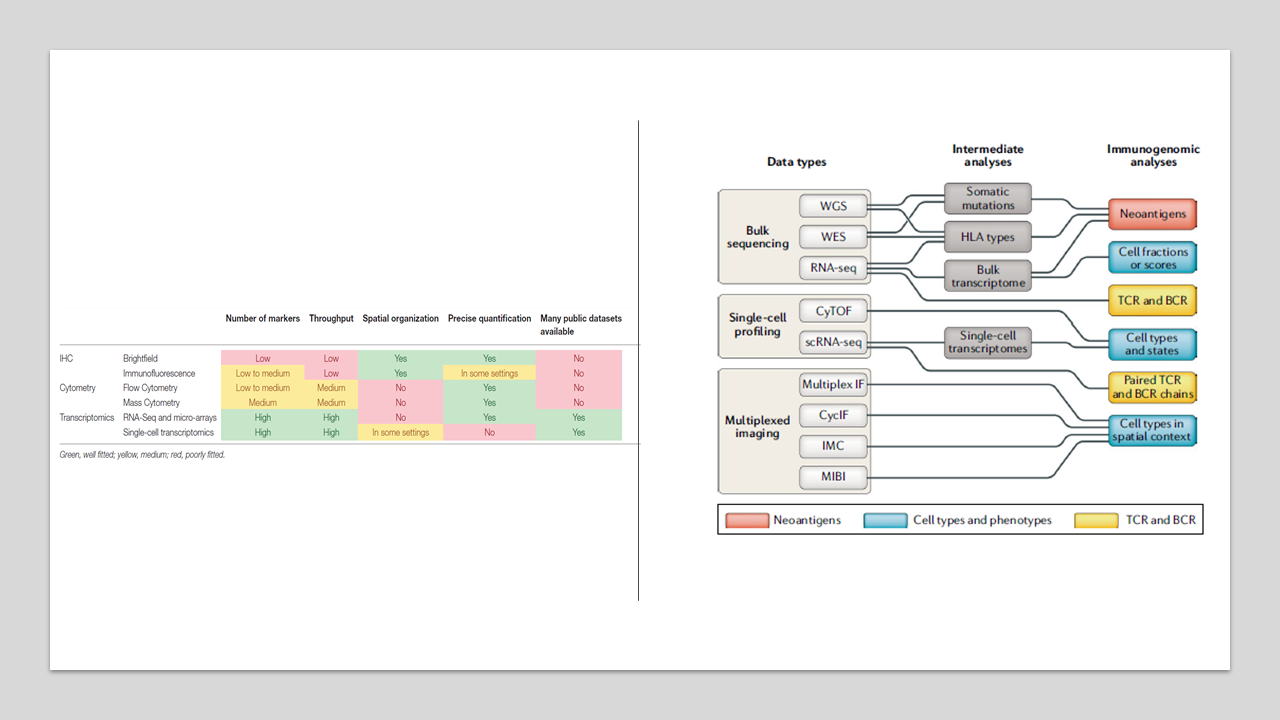
\includegraphics{figures/tme_estimation_technics.PNG} Finotello and
%Trajanoski \autocite{finotello_trajanoski18}








Several emerging promising methods aim at keeping the spatial
information of transcriptomic data along with the origin of identified
tumoral cell types. Using barcodes associated to different regions of
the analysed tissue prior to RNA-Seq, Ståhl et al.~and Salmen et
al.~pioneered the field of Spatial Transcriptomics
\autocite{salmen_etal18}. Recently, the
combination of contrast-enhanced tomography images with RNA-seq data
enabled to identify the radiomic signature of tumour-infiltrating CD8+ T
cells \autocite{sun_etal18}.
Simultaneous measures of distinct omics data, for example joint \acrshort{RNA-Seq}
and epitopes analyses (CITE-seq,
\autocite{stoeckius_etal17}), or
\acrshort{RNA-Seq} and proteomics data (REAP-seq,
\autocite{peterson_etal17}) could
unravel the tumoral cell signalling pathways. Indeed, dysfunctional
tumoral signalling arises from a combination of gene mutations with
epigenetic modifications, inducing rewiring of the signalling network \autocite{yaffe19}.
Additionally, regulation of cell signalling has a strong impact on the
fate of the tumoral clone, intervening in cell growth, cell-cell communications, cell cycle and cell death mechanisms. Last, most of
targeted drugs are directed against signalling molecules, combining them
would require computational predictive analyses of the pharmacological
signalling rewiring. Unfortunately, the crosstalk between oncogenic
signalling and signalling rewiring induced by drugs is still not used in
clinical decision-making due to the lack of reproducibility. And use of
RNA-seq data only as a surrogate of the protemics is suboptimal, as a
large part of the epigenetic regulation of signalling pathways is
performed at the post-transcriptional level. All these approaches could pave the way for non-invasive exploration of tumoral landscape and enable longitudinal monitoring of the effects of immunotherapy.

Alternatively, transferring information from one data set to another,using transfer learning approaches, is helpful to explore partial information. For instance, in study (181),  \acrshort{scrna} was used for cell
type annotation, enabling to reveal finer differences of gene expression
regulation processes spotted by chromatin accessibility data, generated
using sscATAC-seq technics. Last but not least, mathematical mechanistic
modelling provide quantitative predictions that can be experimentally
validated, with pioneered investigation on the dynamics of
tumorigenesis \autocite{iwami_etal12} or the development of Gemini in-silico patient models to predict the effects of combination therapies \autocite{kather_etal18}.



